\chapter{Introduction}

Further development in medical research require insight into complex
systems, that is too complicated to study with mathematical models and
super computers.

Further development in medical sciences cannot only rely on Moore's
law but also improvement on mathematical models and numerical
methods. 

To lower the risk for the patient we need to more accuratley dioagnose
the patient, and find the optimal treatment.

Personalized medican at the level of the individual. 

Many variables to take into account

The story of biomechanics starts in the 17th century with Giovanni
Borelli, known as the father of Biomechanics. He was the first one to
apply the mathematical techniques of Gallileo Galliei to study the
movement of animals. 


\section{Aim of thesis}

The focus of this thesis has been to develop a framework for
constructing patient specific mechanical models of a patients heart. 



%%% Local Variables:
%%% mode: latex
%%% TeX-master: "../../main"
%%% End:

\section{Cardiac Anatomy and Physiology}

The heart is the muscular organ responsible for circulating the blood
thoughout the body. 

Deoxgenated blood transported from the body trough the veins to the
right atrium (RA) 



\subsection{Myocardial structure and morphology}

\subsection{Myocardial Contractility}

%%% Local Variables:
%%% mode: latex
%%% TeX-master: "../../main"
%%% End:

% \section{Mechanical modeling}
\label{sec:intro_mechanical}

In this section we will cover the necessary theory of continuum
mechanics in order to model the mechanics of the heart. The theory of
continuum mechanics is extensive, and we will not be able to cover
everything. For a complete review of continuum mechanics the reader is
therefore referred the textbook of Gerard Holzapfel
\cite{holzapfel2000nonlinear} from which most of the theory in this
section is taken. For the even more mathematically oriented reader we
refer to \cite{marsden1994mathematical}.

\subsection{Kinematics}
We represent the heart as a continuum body $\mathfrak{B}$ embedded in
$\mathbb{R}^3$. A configuration of $\mathfrak{B}$ is a mapping $\chi:
\mathfrak{B} \rightarrow \mathbb{R}^3$. 
We denote the \emph{reference configuration} of the heart by $\Omega
\equiv \chi_0(\mathfrak{B})$, and the \emph{current configuration} by $\omega
\equiv \chi(\mathfrak{B})$. The mapping $\varphi :  \Omega
\rightarrow \omega$, given by the composition $\varphi = \chi
\circ \chi_0^{-1}$, is a smooth, orientation preserving (positive
determinant) and invertible map. We denote the coordinates in the
reference configuration by $\Xvec \in \Omega$, and the coordinates in the current
configuration by $\xvec \in \omega$. The coordinates $\Xvec$ and $\xvec$ are
commonly referred to as material and spatial points respectively, and
are related through the mapping $\varphi$, by $\xvec = \varphi(\Xvec)$.
For time-dependent problems it is common to make  the time-dependence
explicitly by writing $\xvec = \varphi(\Xvec, t)$. In the following
we will only focus on the mapping between two configurations and
therefore no time-dependence is needed. The mapping $\varphi$ will be
referred to as the \emph{motion}. The \emph{deformation gradient} is a
rank-2 tensor, defined as the partial derivative of the motion with
respect to the material coordinates:
\begin{align}
  \F(\Xvec) = \frac{\partial \varphi}{\partial \Xvec} = \Grad \xvec.
  \label{eq:deformation_gradient}
\end{align}
Here we also introduce the notation $\Grad$, which means derivative
with respect to reference coordinates.
The deformation gradient maps vectors in the reference configuration to
vectors in the current configuration, and belongs to the space of
linear transformations from $\mathbb{R}^3$ to $\mathbb{R}^3$ with
strictly positive determinant, which we denote by
$\mathrm{Lin}^+$. Another important quantity is the
\emph{displacement} field  
\begin{align}
  \uvec = \xvec-\Xvec, 
  \label{eq:displacement}
\end{align}
which relates positions in the reference configuration to positions
in the current configuration. From \eqref{eq:deformation_gradient} we
see that
\begin{align}
  \F = \Grad \xvec = \Grad \uvec + \Grad \Xvec = \Grad \uvec + \I.
\end{align}
Some other useful quantities are the \emph{right Cauchy-Green} deformation
tensor $\C = \F^T\F$, the \emph{left Cauchy-Green} deformation tensor
$\mathbf{B} = \F\F^T$, the \emph{Green-Lagrange} strain tensor
$\mathbf{E} = \frac{1}{2}(\C - \I)$, and the determinant of the
deformation gradient $J = \det \F$.

An important concept in mechanics is the concept of stress, which is
defined as force per area
$\left[\frac{\mathrm{N}}{\mathrm{m}^2}\right]$. When working with
different configurations one needs to be careful with which forces and
which areas we are talking about. Table \ref{tab:stress_tensor}
shows how forces and areas are related for the most important stress
tensors used in this thesis. Note that the explicit form of the stress
tensor requires a constitutive law for the material at hand. This will
be discussed in more detail in Section \ref{sec:constitutive_relations}.

\begin{table}[h]
  \centering
  \begin{tabular}{lll}
    \toprule
    Stress tensor & Forces & Area \\
    \midrule
    Second Piola-Kirchhoff ($\SPK$) & Reference configuration & Reference configuration \\
    First Piola-Kirchhoff ($\FPK$) & Current configuration  &  Reference configuration \\
    Cauchy ($\Cauchy$) &  Current configuration & Current configuration  \\
    \bottomrule
  \end{tabular}
  \caption{\label{tab:stress_tensor}Showing different stress tensors
    used in this thesis, and how
    they relate forces to areas trough different configurations.}
\end{table}


\subsection{Balance laws and transformations}
In this section we will cover some basic transformation used to
derive the fore-balance equations for the mechanics of the heart. 

\subsubsection{Transformations between reference and current
  configuration}
By definition, the reference configuration $\Omega$, and current
configuration $\omega$, are related via the motion $\varphi$ in the
sense that a point $\mathfrak{p} \in \mathfrak{B}$ with reference
coordinates $\Xvec$ and current coordinates $\xvec$ satisfies $\xvec =
\varphi(\Xvec)$. Likewise a vector in the reference configuration is
related to a vector in the current configuration  via the
deformation gradient $\F$; if $\mathrm{d}\Xvec$ is a vector in the
reference configuration it will transform to the vector
$\mathrm{d}\xvec$ in the current configuration, and $\mathrm{d}\xvec =
\F \mathrm{d}\Xvec$. From this relation we also derive that the
transformation of an infinitesimal volume element in the reference
configuration, $\mathrm{d}V$ is related to an infinitesimal volume
element in the current configuration, $\mathrm{d}v$  via the determinant of the
deformation gradient,
\begin{align}
  \mathrm{d}v =\det(\F) \mathrm{d}V.
  \label{eq:volume_element}
\end{align}
Another important transformation is the transformation of normal
vectors. By noting that we can write \eqref{eq:volume_element} using
surface elements
\begin{align*}
  \mathrm{d}s \mathbf{n} \mathrm{d}\xvec  &= \mathrm{d}v = \det(\F) \mathrm{d}V = \det(\F) \mathrm{d}S  \Nvec \mathrm{d}\Xvec\\
  &\implies \left( \mathrm{d}s \mathbf{n} \F  - \mathrm{d}S \det(\F) \Nvec \right) \mathrm{d}\Xvec = 0\\
  &\implies \left( \mathrm{d}s \F^T \mathbf{n}  - \mathrm{d}S \det(\F) \Nvec \right) \mathrm{d}\Xvec = 0,\\
\end{align*}
we get \emph{Nanson's formula}
\begin{align}
  \mathrm{d}s \mathbf{n}  =  \det(\F) \F^{-T} \mathrm{d}S \Nvec,
\end{align}
which relates the normal vector in the current configuration to the
normal vector in the reference configuration.


\subsubsection{Conservation of linear momentum}
Newton's seconds law states that the change in linear momentum equals
the net impulse acting on it. For a continuum material with constant
mass density $\rho$ this implies that
\begin{align}
  \int_{\omega} \rho \dot{\mathbf{v}} \mathrm{d}v = \mathbf{f},
  && \mathbf{f} = \int_{\partial \omega} \mathbf{t} \mathrm{d}s
     + \int_{\omega} \mathbf{b} \mathrm{d}v,
     \label{eq:cons_lin_mom}
\end{align}
where $\mathbf{v}$ is the spatially velocity field, $\mathbf{t}$ is
the traction acting on the boundary, and $\mathbf{b}$ is the body
force. From \emph{Cauchy's stress theorem} we know that there exist a
second order tensor $\sigma$, known as as Cauchy stress tensor that is
related to the traction vector by $\mathbf{t} = \sigma \mathbf{n}$,
where $\mathbf{n}$ is the unit normal in the current configuration.
Using the divergence theorem we get.

\begin{align*}
  \int_{\partial \Omega} \mathbf{t} \mathrm{d}s
  = \int_{\partial \Omega} \sigma \mathbf{n} \mathrm{d}s
  = \int_{\Omega} \nabla \cdot \sigma \mathrm{d}v,
\end{align*}
and by collecting the terms from \eqref{eq:cons_lin_mom}. We arrive at
Cauchys momentum equation
\begin{align}
  \nabla \cdot \sigma + \mathbf{b} =  \rho \dot{\mathbf{v}}.
  \label{eq:chauch_momentum_eq}
\end{align}
The contribution from the body force ($\mathbf{b}$)  and inertial term
($\rho \dot{\mathbf{v}}$) are negligible compared to the stresses
\cite{hunter1996kd,tallarida1970left, moskowitz1981effects}, which is
why the force balance equations is typically only stated as
\begin{align}
  \nabla \cdot \sigma = \mathbf{0}.
  \label{eq:momentum_simple_current}
\end{align}
Note that we have formulated the balance law in the current
configuration. An equivalent statement can be formulated in terms of
the reference configuration
\begin{align}
  \nabla \cdot \FPK = \mathbf{0}, 
  \label{eq:momentum_simple_reference}
\end{align}
where $\FPK$ is the first Piola-Kirchhoff stress tensor.

\subsubsection{Conservation of angular momentum}
Just like linear momentum, the angular momentum is also a conserved
quantity. We will not go through the derivation of resulting
equations, but state that as a consequence, the Cauchy stress tensor is
symmetric
\begin{align}
  \sigma = \sigma^T.
\end{align}



\subsection{Hyperelasticity}
\label{sec:hyperelasticity}

Even though experimental studies have indicated a visco-elastic behavior
of the myocardium \cite{dokos2002shear, gultekin2016orthotropic}, a
common assumption is to consider a quasi-static behavior, meaning that
the inertial term in \eqref{eq:chauch_momentum_eq} is negligible and
static equilibrium can be achieved at any time. Therefore
it is also possible to model the myocardium as a hyperelastic material
which is a type of elastic material.
This means that we postulate the existence of
a strain-energy density function $\Psi:\mathrm{Lin}^+ \rightarrow
\mathbb{R}^+$, and that stress is given by the relation
\begin{align}
\FPK = \frac{\partial \Psi(\F)}{\partial \F}.
\end{align}
Since stress has unit Pa, we see that the strain-energy density
function is defined as energy per unit reference volume, and has units
$\frac{\text{Joule}}{m^3}$. 
The strain-energy density function relates  the amount of
energy that is stored within the material in response to a given
strain. Hence, the stresses in a hyperelastic material with a given
strain-energy density function, depends only on the strain, and not the
path for which the material deforms. On the contrary, if the model had
been visco-elastic we would expect to see hysteresis in the
stress/strain curve, but this is not possible for a hyperelastic
material. 

\begin{remark}
  The second law of thermodynamics states that the total entropy
  production in a thermodynamic process can never be negative. Elastic
  materials defines a special class of materials in which the entropy
  production is zero. Within this thermodynamic framework the
  strain-energy density function coincides (up to a constant) with the
  Helmholtz free energy density.
\end{remark}


\subsubsection{General requirements for the strain-energy density
  function}
\label{sec:strain_energy_req}
Some general requirements must hold for the strain-energy function.
First of all, we require that the reference state is stress free and
that the stored energy increases monotonically with the deformation. 
Formally this can be stated simply as 
\begin{align*}
  \Psi(\I) = 0 \; && \text{and} &&\; \Psi(\F) \geq 0.
\end{align*}
Moreover, expanding or compressing a body to zero volume would
require an infinite amount of energy, i.e
\begin{align*}
  \Psi(\F) \rightarrow \infty \; && \text{as} &&\; \det \F \rightarrow& 0 \\
  \Psi(\F) \rightarrow \infty \; && \text{as} &&\; \det \F \rightarrow& \infty
\end{align*}
We say that the strain energy should be objective, meaning that the
stored energy in the material should be invariant with respect to
change of observer. Formally we must have: \emph{given any positive symmetric
rank-2 tensor $\C \in \mathrm{Sym}$:}
\begin{align}
  \Psi(\mathbf{C}) = \Psi(\mathbf{Q}\mathbf{C}\mathbf{Q}^T), \; \forall \mathbf{Q} \in \mathcal{G} \subseteq \mathrm{Orth}.
\end{align}
Here $\mathrm{Orth}$ is the group of all positive orthogonal matrices.
If $\mathcal{G} = \mathrm{Orth}$ we say that the material is
isotropic, and otherwise we say that the material is anisotropic.
This brings us to another important issue, which is related to the
choice of coordinate-system. Having to deal with different
coordinate-systems, and mapping quantities from one coordinate-system
to another can results in complicated computations. Therefore it would be beneficial if we
could work with quantities which do not depend on the choice of
coordinate-system. Such quantities are called invariants. 
If the material is isotropic, the representation theorem for
invariants states that $\Psi$ can be expressed in terms of the
principle invariants of $\mathbf{C}$, that is $\Psi = \Psi(I_1, I_2,
I_3)$. The principle invariants $I_i, i=1,2,3$ are the coefficients in
the characteristic polynomial of $\mathbf{C}$, and is given by 
\begin{align}
  I_1 = \tr \C,  && I_2 = \frac{1}{2}\left[ I_1^2 - \tr(\C^2)\right] && \text{and} && I_3 = \det \C.
\end{align}
In the case when the material constitutes a transversely isotropic
behavior, that is the material has a preferred direction $\mathbf{a}_0$,
which in the case of the myocardium could be the direction of fiber
muscle fibers, we have
\begin{align*}
  \mathcal{G} = \{ \mathbf{Q} \in \mathrm{Orth}: \mathbf{Q}(\mathbf{a}_0\otimes\mathbf{a}_0)\mathbf{Q}^T\},
\end{align*}
with $\otimes$ being the outer product. In this case the strain-energy
density function can still be expressed through invariants. However,
we need to include the so called quasi-invariants, which are defined
as stretches in the local microstructural coordinate-system. The
transversely isotropic invariants are given by
\begin{align*}
  I_{4\mathbf{a}_0 } = \mathbf{a}_0 \cdot (\C \mathbf{a}_0) && \text{and} && I_5 = \mathbf{a}_0 \cdot (\C^2 \mathbf{a}_0).
\end{align*}
The invariants do have a physical interpretation. For instance, $I_3$
is related to the volume ratio of material during deformation, while
$I_{4\mathbf{a}_0 } $ is related to the stretch along the direction
$\mathbf{a}_0 $. Indeed the \emph{stretch} ratio in the direction
$\mathbf{a}_0$ is given by $\lambda_{\mathbf{a}_0} = | \F \mathbf{a}_0
|$ and we see that $I_{4\mathbf{a}_0 }  =  \mathbf{a}_0 \cdot (\C
\mathbf{a}_0) = \F \mathbf{a}_0 \cdot (\F \mathbf{a}_0) =
\lambda_{\mathbf{a}_0}^2$. For more details about invariants see
\cite{holzapfel2009constitutive,liu1982representations}.


The theory of global existence of unique solutions for elastic problem
was originally based convexity of the free energy function.
A function $\phi: \Omega \rightarrow \mathbb{R}$ is \emph{convex} if for any
$\Xvec_1, \Xvec_2 \in \Omega$ we have
\begin{align}
  \phi(\lambda \Xvec_1+ (1-\lambda) \Xvec_2)
  \leq \lambda \phi(\Xvec_1)
  + (1-\lambda) \phi(\Xvec_2).
\end{align}
However, from a physical point of view this requirement is too strict
\cite{ball1976convexity}. A slightly weaker requirement is that the
strain-energy function $\Psi$ is \emph{polyconvex}, meaning that there exist
a convex function $\phi$ such that
\begin{align*}
  \Psi(\F) = \phi(\F, \cof \F, \det \F).
\end{align*}
Note however, that if $\Psi$ is convex then it is also polyconvex.


% \subsubsection{Work conjugates}


% \begin{table}[h]
%   \centering
%   \begin{tabular}{ll}
%     \toprule
%     Stress & Strain \\
%     \midrule
%     Second Piola ($\SPiola$) & Green Lagrange ($\mathbf{E}$) \\
%     First Piola ($\FPiola$) & Deformation gradient ($\mathbf{F}$) \\
%     Cauchy ($\mathbf{\sigma}$) &  Eulerian-Almansi ($\mathbf{e}$) \\
%     \bottomrule
%   \end{tabular}
%   \caption{\label{tab:work_conjugates}Work conjugate stress-strain pairs}
% \end{table}

% By conjuagate stress-strain paris we mean that the rate of mechanical
% work is given by the stress times the strain-rate. For example,
% the total work per unit volume done by the stresses from time $t_1$ to
% $t_2$ is given by
% \begin{align}
%   \mathcal{W}(t_1, t_2) &=  \int_{t_1}^{t_2} \mathbf{P} : \dot{\F} dt
%                           = \int_{t_1}^{t_2} \frac{\partial \Psi (\F)}{\partial \mathbf{F}}  : \dot{\F} - p \F^{-T} :  \dot{\F}  dt \\
%                         &= \int_{t_1}^{t_2} \frac{D \Psi (\F)}{D t} - p\cdot 0 dt
%                           = \Psi(\F(t_2)) - \Psi(\F(t_1)).
% \end{align}
% Note that this is a measure of work per unit volume.


\subsection{Incompressibility}
\label{sec:incompressibility}

The myocardium is composed by small blood vessels that supply the
myocardial cells with oxygen. When the myocardium contracts, this
perfused blood is squeezed out, resulting in an overall loss of
2-4\% volume\cite{yin1996compressibility}. Such materials are
referred to as compressible. When the 
volume are preserved we refer to the material as incompressible.
Since 2-4\% is very little, a common assumption in cardiac mechanical modeling,
which has also been made in the work conducted in this thesis, is to assume
the myocardium to be incompressible. The reason for this choice is
purely numerical.

For an incompressible material, only isochoric motions are
possible. This means that volume of the material do not change during
any deformation and hence we have the constraint 
\begin{align}
  J = \det(\F) = 1.
  \label{eq:incompressible_cons}
\end{align}
The constraint \eqref{eq:incompressible_cons} can be imposed by
considering the modified strain energy function
\begin{align}
  \Psi = \Psi(\F) + p(J-1),
  \label{eq:incomp_strain_energy}
\end{align}
where $p$ is a scalar which serves as a Lagrange multiplier, but which
can be identified as the hydrostatic pressure. If we differentiate
\eqref{eq:incomp_strain_energy} with respect to $\F$ we get the First
Piola-Kirchhoff stress tensor for an incompressible material
\begin{align}
  \FPK = \frac{\partial \Psi(\F)}{\partial \F} + J p \F^{-T}.
\end{align}
Likewise the Cauchy stress tensor is given by
\begin{align}
  \Cauchy = J^{-1} \frac{\partial \Psi(\F)}{\partial \F}\F^{T} + p \I.
  \label{eq:cauchy_incomp}
\end{align}


\begin{remark}
  The sign of $p$ is determined by whether you add or subtract the term
  $ p(J-1)$ to the total strain energy in
  \eqref{eq:incomp_strain_energy}. For all practical purposes, it
  does not matter if you add or subtract the term as long as you are
  consistent. 
\end{remark}


\subsubsection{Uncoupling of volumetric and isochoric response}
The total strain energy function in \eqref{eq:incomp_strain_energy}
can be written as a sum of isochoric and volumetric components. Let
\begin{align}
  \F =  \F_{\mathrm{vol}} \F_{\mathrm{iso}},
\end{align}
then $ \F_{\mathrm{vol}} =
J^{1/3}\I$ and $\F_{\mathrm{iso}} = J^{-1/3}\F$. For
compressible material (i.e with $J \neq 1$) it is important to consider
only deviatoric strains in the strain-energy density function, so that
$\Psi = \Psi_{\mathrm{iso}}(\F_{\mathrm{iso}}) +
\Psi_{\mathrm{vol}}(J)$. For incompressible material ($J = 1$), we
have $\F_{\mathrm{vol}} = \I$ so that such a decomposition seems
unnecessary. However, a similar decomposition has shown to be
numerically beneficial \cite{weiss1996finite}. Note that, in this case, a similar
decoupling of the stress tensors has to be done.

\subsection{Boundary Conditions}
\label{sec:mech_boudary}


Choosing the correct boundary conditions for the model is essential,
and the choice should mimic what is observed in the reality. To
physiologically constrain the ventricle in a correct way is difficult,
and different approaches has been proposed.
The boundary condition at the endocardium is typically modeled as a
Neumann boundary condition, representing the endocardial blood
pressure. For the left ventricle we have
\begin{align}
  \sigma \mathbf{n} = -p_{\mathrm{lv}} \mathbf{n}, \;  \xvec \in  \lVendoCur, 
\end{align}
and for the right ventricle, ``lv'' is substituted with ``rv''.
This condition has a negative sign because the unit normal
$\mathbf{N}$ is pointing out of the domain, while the pressure is
acting into the domain. 
Note that this condition is imposed on the current configuration, and
to utilize the Lagrangian formulation we can pull back this condition
to the reference configuration to obtain
\begin{align}
  \FPK\mathbf{N} &= -p_{\mathrm{lv}} J\mathbf{F}^{-T} \cdot \mathbf{N}, \;  \Xvec \in \lVendo
\end{align}
Likewise, it is common to enforce a
Neumann boundary condition on the epicardium,
\begin{align}
\FPK\mathbf{N}  &= -p_{\mathrm{epi}}  J\mathbf{F}^{-T} \cdot \mathbf{N}, \;  \Xvec \in \epi.
\end{align}
However, the pressure $p_{\mathrm{epi}}$ is usually set
to zero.

There exist a variety of boundary conditions at the base.
It is common to constrain the longitudinal motion of
base, even though it is observed in cardiac images that the apex tend
to be more fixed than the base. A recent study shows that taking into
account the base movement is important to capture the correct
geometrical shape \cite{palit2016passive}. However, this has not been
done in the studies in this thesis.
Fixing the longitudinal motion at the base is enforced through a
Dirichlet boundary condition,
\begin{align}
  u_1 = 0,  \;  \Xvec \in \lvbase,
\end{align}
where $u_1$ is the longitudinal component of the displacement $\uvec =
(u_1, u_2, u_3)$. To apply this type of condition, it is easiest if
the base is flat and located at a prescribed location, for example in
the $x= 0$ plane. Constraining the longitudinal motion of the base
alone is not enough since the ventricle is free to move in the basal
plane. In order to anchor the geometry it is possible to fix the
movement of the base in all directions
\begin{align}
  \uvec = \mathbf{0},  \;  \Xvec \in \lvbase,
\end{align}
or fixing the endocardial or epicardial ring
\begin{align}
  \uvec &= \mathbf{0},  \;  \Xvec \in \Gamma_{\mathrm{endo}} \\
  \uvec &= \mathbf{0},  \;  \Xvec \in \Gamma_{\mathrm{epi}}.
\end{align}

Another approach which is used in this thesis is to impose a Robin
type boundary condition at the base
\begin{align}
  \FPK \Nvec + k \uvec = \mathbf{0},  \;  \Xvec \in \lvbase, 
\end{align}
or at the epicardium to mimic the pericardium
\begin{align}
  \FPK \Nvec + k \uvec = \mathbf{0},  \;  \Xvec \in \lvepi, 
\end{align}
Here $k$ can be seen as the stiffness of a spring that limit the
movement. The limiting cases, $k = 0$ and $k \rightarrow
\infty$ represent free and fixed boundary respectively.
More complex boundary conditions to mimic the pericardium is also
possible \cite{fritz2014simulation}, but not considered in this thesis.
An overview of the location of the different boundaries for the
bi-ventricular geometry is illustrated in Figure \ref{fig:boundaries}.

\begin{figure}[htbp]
  \centering
    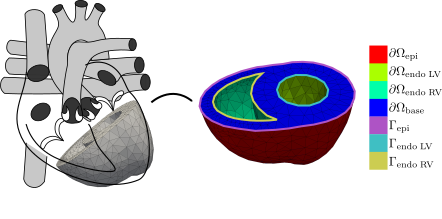
\includegraphics[width=\textwidth]{chapters/introduction/figures/boundaries}
\caption{Illustration of the different boundaries in a bi-ventricular
  domain.}
\label{fig:boundaries}
\end{figure}


\subsection{Force-balance equation}
We will now collect all the terms that makes up to force balance for
the cardiac mechanics problem. Considering the myocardium as a incompressible,
hyperelastic material with a Robin type boundary condition at the base
we obtain the following strong form in the Lagrangian formulation
\begin{align}
  \begin{split}
  \nabla \cdot \FPK &= 0 \\
  J - 1 &= 0,
  \end{split}
 \label{eq:force_balance_strong}
\end{align}
completed with appropriate boundary conditions. To solve this
numerically using the finite element method, we need to derrive weak
variational form of this equaiton.
% \begin{align}
%   \FPK \Nvec + k \uvec &= \mathbf{0},  \;  \Xvec \in \lvbase\\
%   u_1 &= 0,  \;  \Xvec \in \lvbase \\
%   \FPK\mathbf{N}  &= \mathbf{0}, \;  \Xvec \in \epi \\
%   \FPK\mathbf{N} &= -p_{\mathrm{lv}} J\mathbf{F}^{-T} \cdot \mathbf{N}, \;  \Xvec \in \lvendo
%   \label{eq:bndry_conditions_strong}
% \end{align}
 


\subsubsection{Variational formulation}
\label{sec:variational_formulation}
There are many ways to arrive at the variational formulation of the
force-balance equations for the cardiac mechanics problem.  One way is
to consider the strong form in \eqref{eq:force_balance_strong} and use
the standard approach in the finite element method to multiply by
test function in a suitable space, and perform integration by
parts. Within the fields of continuum mechanics it is common to
refer to this approach as the \emph{principle of virtual work}, with states
that the virtual work of all forces applied to a mechanical system
vanishes in equilibrium. Within this framework, test functions are
referred to as virtual variations.
Another approach, which we will use here, derives the variational form
by utilizing a fundamental principle in physics
called the \emph{principle of stationary potential energy}, or
\emph{minimum total potential energy principle}. This principle states that a
physical system is at equilibrium when the total potential energy is
minimized, and any infinitesimal changes from this state should not add
any energy to the system.
In order to make use of this principle we first need to sum up all the
potential energy in the system. Here we separate between internal and
external energy. Internal energy, is energy that is stored within the
material, for instance when you stretch a rubber band you increase its
internal energy. External energy represent the contribution from all
external forces such as gravity and traction forces.
% We consider the equilibrium in the referece domain, and denote the
% domain of interest by $\Omega \subset \mathbb{R}^3$, with boundary
% $\partial \Omega$. For the case of a left ventrcular domain we have
% $\partial \Omega = \lvendo \cup \lvepi \cup \lvbase$ and for a
% bi-ventricular domain we include $\rvendo$ in the partition as well. 
For a hyperelastic and incompressible material, the total potential
energy in the system is given by
\begin{align}
  \Pi(\uvec, p) &= \Pi_{\mathrm{int}}(\mathbf{u},p) + \Pi_{\mathrm{ext}}(\mathbf{u}). \\
  \Pi_{\mathrm{int}}(\uvec,p) &= \int_{\Omega} \left[ p(J - 1) +  \Psi(\mathbf{F}) \right] \mathrm{d}V\\
  \Pi_{\mathrm{ext}}(\mathbf{u}) &= - \int_{\Omega} \mathbf{B} \cdot \mathbf{u} \mathrm{d} V - \int_{\partial \Omega_N} \mathbf{T} \cdot \mathbf{u} \mathrm{d}S
\end{align}
Here $\mathbf{B}$ represents body forces acting on a volume element in
the reference domain, e.g  gravity, and $\mathbf{T} = \mathbf{P}
\mathbf{N}$ represents first Piola-Kirchhoff traction force acting on
the Neumann boundary $\partial \Omega_N$. According to the
\emph{Principle of stationary potential energy} we have  
\begin{align}
  D_{\delta \mathbf{u}} \Pi(\mathbf{u}, p) = 0,  && \text{and} && D_{\delta p} \Pi(\mathbf{u}, p) = 0.
  \label{eq:minimum_potential_energy}
\end{align}
Here $\delta \mathbf{u}$ and $\delta p$ are virtual variations in the
space for the displacement and hydrostatic pressure respectively, and
\begin{align}
  D_{\mathbf{v}} \Phi(\mathbf{x}) = \frac{\mathrm{d}}{\mathrm{d}\varepsilon} \Phi(\mathbf{x} + \varepsilon \mathbf{v})\big|_{\varepsilon = 0}
\end{align}
is the directional derivative of $\Phi$ at $\mathbf{x}$ is the
direction $\mathbf{v}$. This operator is also known as the G\^ateaux
operator. The virtual variations $\delta \mathbf{u}$ and $\delta p$
represents an arbitrary direction with infinitesimal magnitude. We have
\begin{align}
  0 = D_{\delta p} \Pi(\mathbf{u}, p)
  = \int_{\Omega}  \delta p(J(\mathbf{u}) - 1) \mathrm{d}V,
\end{align}
and
\begin{align*}
  \begin{split}
  0 = D_{\delta \mathbf{u}} \Pi(\mathbf{u}, p) 
  =&  \int_{\Omega}  \left[ pJ \mathbf{F}^{-T} + \mathbf{P} \right] : \Grad \delta \mathbf{u} \mathrm{d}V - \int_{\Omega} \mathbf{B} \cdot \delta \mathbf{u} \mathrm{d} V
  \end{split}
\end{align*}
Note that the traction forces are now incorporated into the stress
tensors after application of the divergence theorem. These equations
are also commonly referred to as the Euler-Lagrange equations. Here $\uvec  \in V = 
\left[H_D^1(\Omega)\right]^3$, with $H_D^1(\Omega) = \{ \mathbf{v}:
\int_{\Omega} \left[ |\mathbf{v}|^2 +  |\Grad \mathbf{v}|^2
\right]\mathrm{dV} < \infty \wedge \mathbf{v}\big|_{\partial \Omega_D}
= 0\}$ and $p \in Q = L^2(\Omega)$, with $\partial \Omega_D$
representing the Dirichlet boundary. In summary, the Euler-Lagrange
equations written in a mixed form reads : \emph{Find $(\uvec, p)\in V
  \times Q$ such that} 
\begin{align}
  \begin{pmatrix}
    D_{\delta p} \Pi(\mathbf{u}, p)\\
    D_{\delta \mathbf{u}} \Pi(\mathbf{u}, p) 
  \end{pmatrix}
  = \mathbf{0}.  && \forall \; (\delta \uvec, p) \in V \times Q.
 \label{eq:intro_variational_form}
\end{align}


\subsubsection{Discretization of the force balance equations}

Equation \eqref{eq:force_balance_strong} is only possible to solve
analytically for very simplified problems. Therefore we need to employ
a numerical approximation method to solve the problem. One such method
is the finite element method (FEM). When using the finite element method, we often refer to such
approximation as a Galerkin approximation. This is based on
approximating the solution by linear combinations of  basis functions in a finite dimensional
subspace of the true solution. If $V$ and $Q$ are two suitable Hilbert
spaces for the displacement $\uvec$ and the hydrostatic pressure $p$
respectively (see Section \ref{sec:variational_formulation}), we now
select some finite dimensional subspaces $V_h \subset V$ and $Q_h
\subset Q$, which are spanned by a finite number of basis functions.


For incompressible problems such as \eqref{eq:force_balance_strong}, we cannot choose the
approximation spaces $V_h, Q_h$ at random. A known numerical issue
that arises for such saddle-point problems is \emph{locking}, which can be
seen if the material do not deform even if forces are applied. The
problem is solved by requiring the finite element approximation to
satisfy the discrete inf-sup condition \cite{le1982existence}. There
exist several mixed elements that satisfies this condition
\cite{chapelle1993inf}. The elements used in this thesis are the
Taylor-Hood finite elements \cite{taylor1973numerical}. Let the domain of
interest be denoted by $\Omega$, and let $\mathcal{T}_h$ be a
triangulation of that domain in the sense that $\bigcup_{T \in
  \mathcal{T}_h} T = \overline{\Omega}$. Denote by $\mathcal{P}_k
(T)$, the linear space of all polynomials of degree $\leq k$ defined
on $T$. Then for $k \geq 2$, the Taylor-Hood finite element spaces are the spaces
\begin{align}
  V_h = \{  \phi \in C(\Omega) \;  | \; \phi \big| T  \in \mathcal{P}_k (T) , T \in \mathcal{T}_h \},\\
  Q_h = \{  \phi \in C(\Omega) \;  | \; \phi \big| T  \in \mathcal{P}_{k-1} (T) , T \in \mathcal{T}_h \},
\end{align}
where $C(\Omega)$ denotes the space of continuous function on
$\Omega$. In this thesis we have exclusively used these elements with
$k = 2$.



\begin{remark}
  The basis functions that span the Taylor-Hood
  finite element spaces are also known as the
  Lagrangian basis functions. These basis functions, of
  degree $n$, are a polynomials of degree $n$ on each element, but only
  continuous at the nodes (i.e not continuously
  differentiable). Consequently, differentiating a function that is
  expressed as a linear combination of the Lagrangian basis functions,
  will not be continuous at the nodes, and therefore caution has to
  be made when evaluating features that depends on the derivative of
  such functions. Examples of such features are stress and
  strain with depends on the deformation gradient which again depends
  on the derivative of the displacement. One way to deal with this
  issue is to 1) use other types of elements that are continuously
  differentiable everywhere,  such a the cubic Hermite elements or 2) evaluate the features at the
  Gaussian quadrature points where there is no problem with continuity.
\end{remark}


\subsection{Constitutive relations}
\label{sec:constitutive_relations}
We have now covered a mechanical framework which holds any for
material in general. What differentiate the mechanics of soft
living tissue, like the myocardium, from other materials is the
constitutive relations which describes the response of a material to
applied load. Such constitutive relations often comes from
experimental observations, both on observation of anatomical structure
but also from experiments done on tissue slabs.

We have already covered the theory of hyperelasticity and incompressibility in Section
\ref{sec:hyperelasticity} and \ref{sec:incompressibility} respectively
which are types of constitutive relations. In this section we will
cover constitutive relations which only apply to soft living tissue
such as the myocardium. 

A complete constitutive model of the mechanical behavior of the
myocardium must account for both the passive and the active response
of the myocardium.


\subsubsection{Modeling of the passive myocardium}

The passive response of the myocardium has been investigated through
uni-axial, bi-axial and shear deformation experiments \cite{dokos2002shear}.
% Look at Humprey Continuum biomechanics of
% soft biological tissues
In 2009 Holzapfel and Ogden proposed an orthotropic constitutive model
of the passive myocardium \cite{holzapfel2009constitutive} which is
based on the experiments done in \cite{dokos2002shear}. The model
assumes a local orthonormal coordinate system with the fiber axis
$\ef$, sheet axis $\eS$ and sheet-normal axis $\en$. %The subscript
% refers that the vectors $(\ef, \eS, \en)$ are vectors in the reference
% configuration.
From this coordinate system we define the invariants
\begin{align}
  \begin{split}
    I_1 &= \tr(\C) ,\\
    I_{4\ef} &= \ef \cdot (\C \ef),\\
    I_{4\eS} &= \eS \cdot (\C \eS),\\
    I_{8\ef\eS} &=  \eS \cdot (\C \ef), 
  \end{split}
\end{align}
Here $I_{4\ef} $ and $I_{4\eS}$ are the stretches along the
fiber, sheet axis respectively and $I_{8\ef\eS}$ is
related to the angle between the fiber and sheets in the current
configuration given that they are orthogonal in the reference
configuration. Note that since $(\ef, \eS, \en)$ is an orthonormal
system, we have the relation $I_1 = I_{4\ef} + I_{4\eS} +I_{4\en}$,
and so $I_{4\en}$ is redundant. The orthotropic Holzapfel and Ogden
model reads
\begin{align}
  \label{eq:holzapel_full}
  \begin{split}
  \Psi(I_1, I_{4\ef},  I_{4\eS},  I_{8\ef\eS}) =& \frac{a}{2 b} \left( e^{ b (I_1 - 3)}  -1 \right)\\
  +& \frac{a_f}{2 b_f} \left( e^{ b_f (I_{4\ef} - 1)_+^2} -1 \right) \\
  +& \frac{a_s}{2 b_s} \left( e^{ b_s (I_{4\eS} - 1)_+^2} -1 \right)\\
  +& \frac{a_{fs}}{2 b_{fs}} \left( e^{ b_{fs} I_{8\ef\eS}^2} -1 \right).
\end{split}
\end{align}
Here $( x )_+ = \frac{1}{2} \left( x + |x| \right)$, so that the
the terms involving $I_{4\ef}$ and $I_{4\eS}$ only contribute to the
stored energy during elongation. From \eqref{eq:holzapel_full} we see
that it is easy to identify the physical meaning of each term. For
example the first term represents the isotropic contribution which is
the overall stiffness in the extracellular matrix while the second
term accounts for the extra stiffness along the fibers when they are
elongated. It is also straight forward to prove that the strain-energy
function is convex, and that the requirements for existence and
uniqueness discussed in Section \ref{sec:strain_energy_req} are
fulfilled.

In this thesis we have in several occasions used a
transversely isotropic version of \eqref{eq:holzapel_full} which is
obtained by setting $a_{fs} = b_{fs}= a_s = b_s = 0$, i.e
\begin{align}
  \label{eq:holzapel_trans}
  \begin{split}
  \Psi(I_1, I_{4\ef}) = \frac{a}{2 b} \left( e^{ b (I_1 - 3)}  -1 \right)
  + \frac{a_f}{2 b_f} \left( e^{ b_f (I_{4\ef} - 1)_+^2} -1 \right).
  \end{split}
\end{align}
If we further set $a_f = b_f = b = 0$ so that in $a$ is the
only nonzero parameter, then the Holzapfel-Ogden model reduces (after a
series expansion of the exponential and a limiting argument) to
\begin{align}
  \Psi(I_1)  = \frac{a}{2} \left( I_1 - 3 \right), 
\end{align}
which is the model of a Neo Hookean material. The Cauchy stress can be derived
analytically from \eqref{eq:holzapel_full}, by using the chain rule and
\eqref{eq:cauchy_incomp}, 
\begin{align}
  \begin{split}
    J\Cauchy
    =& \frac{\partial \Psi(\F)}{\partial \F}\F^{T} + p \I
    = \sum_{i \in \left\{ 1, 4\ef,  4\eS,  8\ef\eS \right\} }
    \psi_i \frac{\partial I_i}{\partial \F}\F^{T} + p \I \\
    =& p \I + a \left( e^{ b (I_1 - 3)}  -1 \right) \mathbf{B} 
    + 2 a_f (I_{4\ef} - 1)_+  e^{ b_f (I_{4\ef} - 1)^2} \mathbf{f} \otimes \mathbf{f} \\
    &+ 2 a_f (I_{4\eS} - 1)_+  e^{ b_f (I_{4\eS} - 1)^2} \mathbf{s} \otimes \mathbf{s} 
    + a_{fs} I_{8\ef\eS}  e^{ b_{fs} I_{8\ef\eS}^2} \left( \mathbf{f} \otimes \mathbf{s}  +  \mathbf{s} \otimes \mathbf{f} \right),
  \end{split}
\end{align}
where $\mathbf{B} = \F \F^{T}$ is the left Cauchy-Green tensor,
$\mathbf{f} = \F \ef$ and $\mathbf{s} = \F \eS$.

\subsubsection{Modeling of the active contraction}
  

One feature that separate the myocardium from other hyperelastic
materials such as rubber, is its ability to actively generate force
without external loads. This active component of the model can be
incorporated using two fundamentally different approaches known as the
\emph{active stress} and \emph{active strain} formulation.


% As discussed 
% in Section \ref{sec:ventricular_pumping_function}, the myocardium
% contracts in a cyclic manner. 

% There are basically two main approaches to model the active response
% of the myocardium; the \emph{active stress} and the \emph{active strain}
% formulation.

\begin{figure}[htbp]
  \centering
    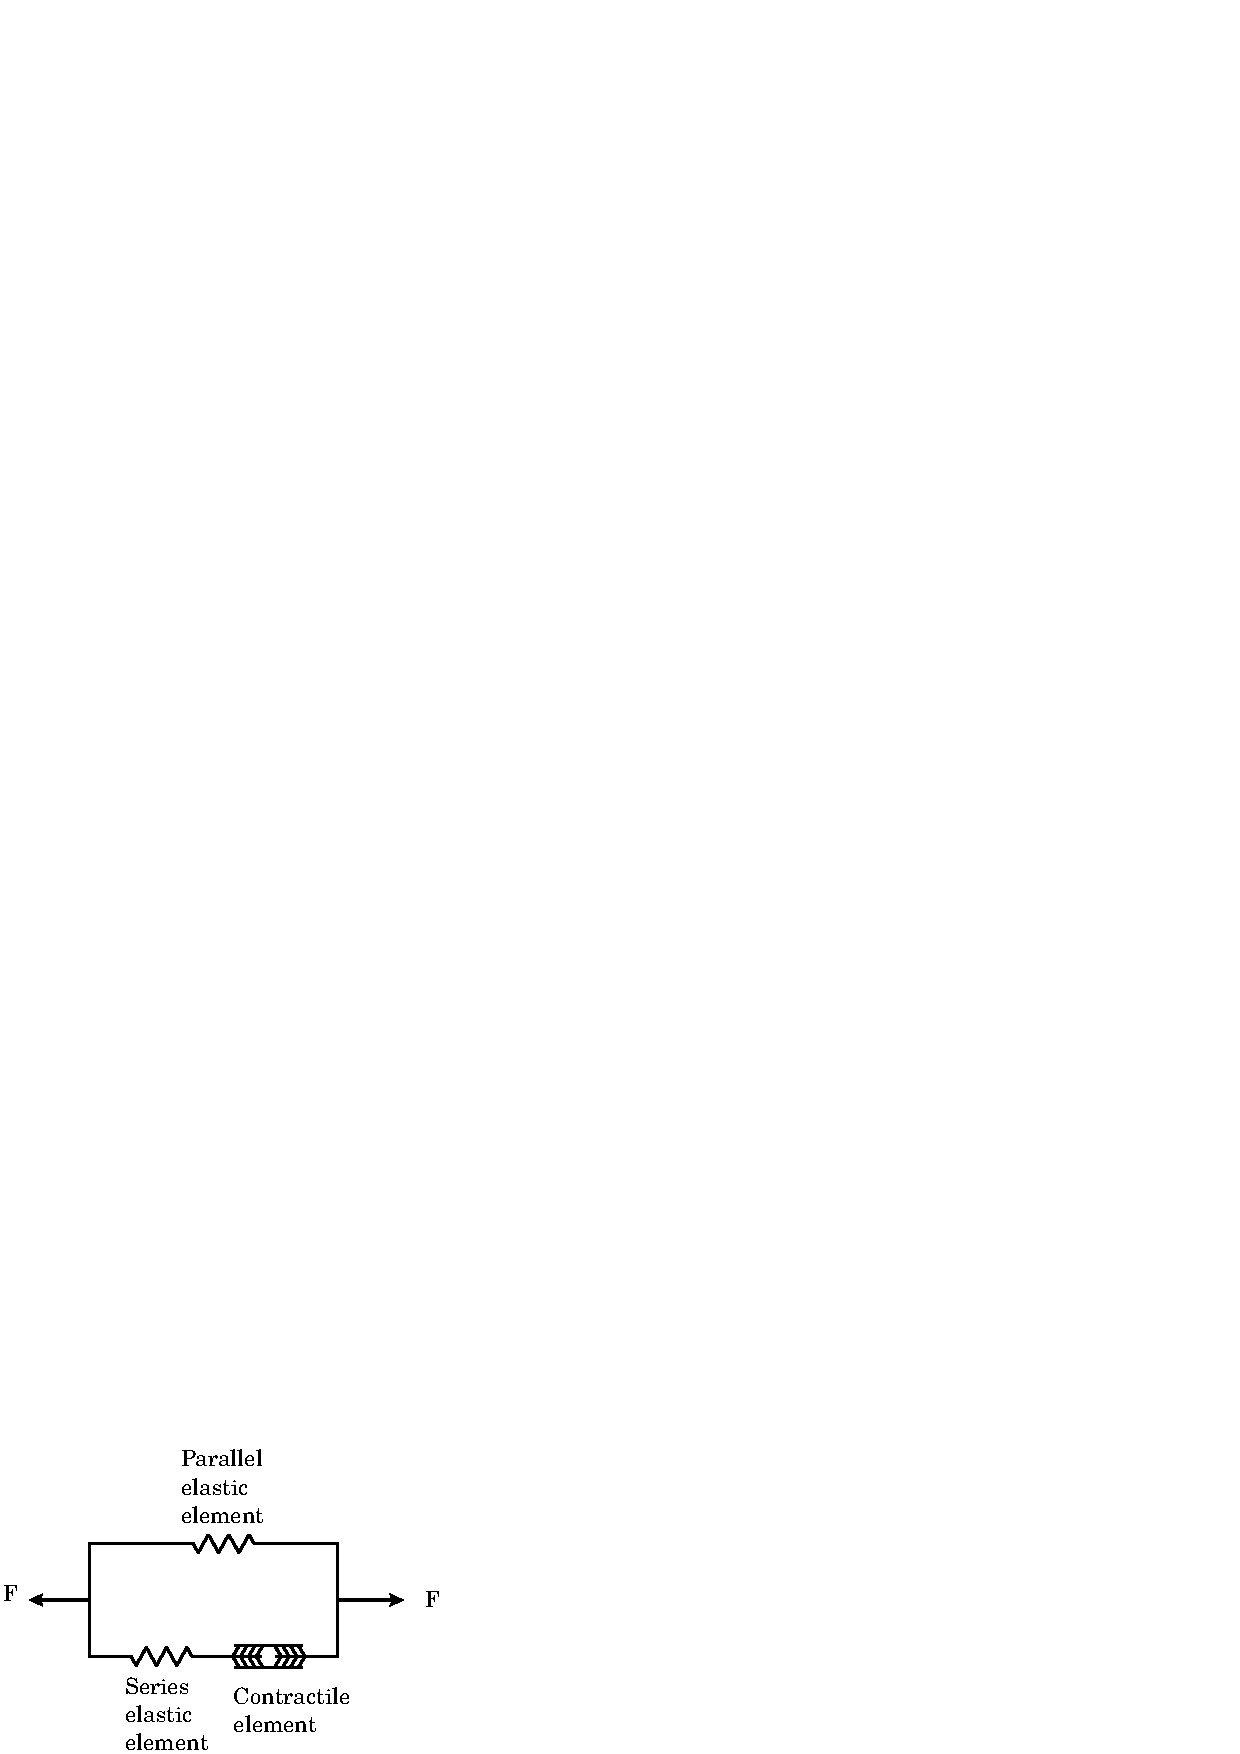
\includegraphics[width=0.5\textwidth]{chapters/introduction/figures/Hill_muscle_model.pdf}
\caption{The classical three-element Hill muscle model with one
  contractile element and two non-linear springs, one arranged in
  series and one parallel. }
\label{fig:hill_muscle_model}
\end{figure}



The active stress approach is based one the classical three element
Hill model illustrated in Figure \ref{fig:hill_muscle_model}, where the
active contribution naturally decomposes the total stress into a sum
of passive and active stresses
\cite{nash2004electromechanical}. Hence, in the active stress
formulation \cite{hunter1998modelling} one assumes that the total
Cauchy stress $\Cauchy$ can be written as an additive sum of one
passive contribution $\Cauchy_p$ and one active contribution $\Cauchy_a$,
\begin{align}
  \Cauchy = \Cauchy_p + \Cauchy_a && J \Cauchy_p =  \frac{\partial \Psi(\F)}{\partial \F} \F^{T}.
\end{align}
The passive contribution is determined by the material model used,
while the active contribution is given by 
\begin{align}
  \Cauchy_a = \Cauchy_{ff} \Fef \otimes \Fef +
  \Cauchy_{ss} \mathbf{s} \otimes \mathbf{s} +
  \Cauchy_{nn} \mathbf{n} \otimes \mathbf{n},
\end{align}
and the different constants $\Cauchy_{ff}, \Cauchy_{ss}$, and
$\Cauchy_{nn}$, which are the active stress in the fiber, sheet and
sheet-normal direction respectively, are typically coupled to the
electrophysiology and calcium dynamics.
There are experimental evidence that the active stresses in the
transverse direction of the fibers ($\Cauchy_{ss}$, and $\Cauchy_{nn}$),
are non-negligible \cite{lin1998multiaxial}, and one approach is to assume
a uniform transverse activation in which the total active tension
can be written as 
\begin{align}
  \Cauchy_a = T_a \left[\Fef \otimes \Fef +
   \eta\left( \mathbf{s} \otimes \mathbf{s} +
  \ \mathbf{n} \otimes \mathbf{n} \right)\right],
  \label{eq:intro_active_stress}
\end{align}
where $\eta$ represent the amount of transverse activation and $T_a
\in \mathbb{R}$ is the magnitude of the active tension.
In the limiting case ($\eta = 0.0$), the active tension acts purely
along the fibers and is reduced to 
\begin{align}
  \Cauchy_a = T_a \Fef \otimes \Fef.
\end{align}
Note that, by observing  that
\begin{align*}
  \frac{\partial I_{4\mathbf{a}_0}}{\partial \F} = \frac{\partial (\mathbf{a}_0  \cdot \C \mathbf{a}_0 )}{\partial \F}
  = 2 \mathbf{a} \otimes \mathbf{a}_0 \implies  \mathbf{a} \otimes  \mathbf{a}= \frac{1}{2} \frac{\partial I_{4\mathbf{a}_0}}{\partial \F} \F^{T}
\end{align*}
and that $I_1 =  I_{4\ef} +  I_{4\eS} +  I_{4\en}$, 
we can instead decompose the strain-energy function into a passive and active
parts \cite{pathmanathan2010cardiac}, $\Psi= \Psi_p + \Psi_a$, with
\begin{align}
\Psi_a = \frac{T_a}{2J} \left(( I_{4\ef} - 1)  + \eta \left[ (I_1 - 3) -
    (I_{4\ef} - 1)\right] \right), 
\end{align}
so that $J \Cauchy_a  = \frac{\partial \Psi_a}{\partial \F}
\F^{T}$.

The active strain formulation is a relatively new way of modeling the
active contraction in the heart and was first introduced in
\cite{taber2000modeling}. This formulation is based on a
multiplicative decomposition of the deformation gradient, 
\begin{equation}
 \F = \F_e \F_a.
\label{eq:active_strain}
\end{equation}


The active part $\F_a$, is an inelastic process driven by the
biochemistry and can be seen as the actual distortion of the
microstructure. The elastic part $\F_e$ is responsible for preserving
compatibility of the tissue and stores all the energy in the
deformations. As a consequence, the strain energy function is a
function of the elastic deformation gradient only $\F_e$. The
decoupling can illustrated by considering two sarcomeres connected in
series as shown in Figure \ref{fig:actstrain}. 

\begin{figure}[htbp]
  \centering
    \includegraphics[width=0.7\textwidth]{chapters/introduction/figures/actstrain.pdf}
\caption{Illustration of the active strain formulation. During the active
deformation, the sarcomeres shortens as if they were all detached. The
elastic deformation ensures compatibility of the tissue.}
\label{fig:actstrain}
\end{figure}


The general form of the active deformation gradient for a
material with an orthotropic active response is given by
\begin{equation}
  \F_a =  \I
  - \gamma_f \ef \otimes \ef
  - \gamma_s \eS \otimes \eS
  - \gamma_n \en\otimes \en
 \label{eq:active_strain_Fa_general}
\end{equation}

We add the constraint $\det(\F_a) = 1$, meaning that the active
deformation is volume preserving. Further we assume that the activation is
transversely isotropic, so that the sheet and sheet-normal axis is
treated in the same way. It is then straight forward to verify that
$\gamma_n = \gamma_s =1- (1-\gamma_f)^{-1/2}$, and we have
\begin{equation}
  \F_a = (1 - \gamma) \ef \otimes \ef  + \frac{1}{\sqrt{1 - \gamma}} (\I - \ef \otimes \ef), 
 \label{eq:intro_active_strain_Fa_gjerald}
\end{equation}
where we set $\gamma = \gamma_f$ for convenience. 


While the motivation behind the active stress formulation is purely
physiological and based on the classical Hill model shown in Figure
\ref{fig:hill_muscle_model}, the motivation behind the active strain
formulation is more driven by ensuring mathematical robustness. In
particular it has been shown \cite{ambrosi2012active} that with the
active strain formulation, properties such as frame invariance and
rank-one ellipticity is inherited from the strain energy function. In
contrast, rank-one ellipticity is not guaranteed for the active stress
formulation.  

% Other types of active models also exists \cite{goktepe2014generalized}
% but will not be discssed f




\subsection{Implementation details}
The cardiac mechanics solver developed during the work of this thesis
is implemented using the finite element framework FEniCS. Here we
briefly explain the main components of FEniCS as well as some
numerical considerations made when implementing the solver.




% A word about FEniCS and how we can implement this
% Newtons method, good initial guess, increment pressure.
% Relatively small system, dense matrix, plot stiffness matrix, Direct
% solver.
% FEniCS compilation stored in cache.
% Fibers at quadrature points. Symbolic language.

\subsubsection{The FEniCS Project}
\label{sec:fenics}

The FEniCS project is an open-source computing platform for solving
partial differential equations (PDEs) using the finite element method (FEM).
Solving PDEs using FEM involves many implementation details that can
be tedious to implement yourselves. The idea behind FEniCS is to
automate code generation so that the user can spend more time on doing
research and less time on implementation of assembly matrices. At the
core of FEniCS is DOLFIN \cite{logg2012dolfin}, which is C++/Python
library, and works as the main interface in FEniCS. In this thesis
only the Python interface has been used, in which C++ code is
automatically generated using SWIG. This allows for simplicity through
the Python scripting language and the speed of the C++ language.
The domain specific language used to represent weak formulations is
called the Unified form language (UFL) \cite{alnaes2014unified}, and
allows for e.g automatic differentiation of forms and expressions. The
FEniCS form compiler (FFC) \cite{logg2012ffc} compiles code written in
UFL to Unified Form-assembly Code (UFC) \cite{alnaes2012ufc} which are
optimized C++ code. The Python interface also makes use of the Instant
module which allows for just-in-time (JIT) compilation of C++
code. The compiled code is also stored in a cache so that compilation
of a form only happens once. Also, the relatively new UFL Analyser and
Compiler System (UFLACS) allows for fast compilation of complex forms
such as forms such as variational formulations that include the Holzapfel
Ogden material model \eqref{eq:holzapel_full}.

For more information about FEniCS, the reader is referred to the
official web page (\url{https://fenicsproject.org}) or any of the
cited literature.

\subsubsection{Numerical considerations}
The solution of non-linear problems such as the one described here is
typically solved using methods like Newton's method. The convergence of
such methods depends on the initial guess, and if the
initial guess is too far from the solution, the solver might diverge.
Moreover, if the initial guess is close to the solution the
convergence rate is in general quadratic.

Let us consider a
typical numerical problem of inflating the ventricular geometry from a
stress-free configuration to end-diastole. This involves increasing
the pressure, or the boundary traction on the endocardium, from zero
to the end-diastolic pressure. A strategy know as the
\emph{incremental load} technique is usually a good approach. In this
strategy you select some incremental step-size (for instance $0.4$
kPa), and increase the pressure linearly until the target pressure is
reached. If the solver diverges you decrease the step-size (for
instance by a factor of 0.5) until convergence is reached, and
continue to step up the pressure with the new step-size. This is very
robust, but definitely a slow approach. Since many of the 
constitutive models for myocardium consist of an exponential
relationship between the stress and strain (so called Fung-type
relation), the amount of stress needed to displace a material will be
higher if the material is a state with high strain compared to a state
of low strain. Therefore, the Newtons solver might perform less
iterations to reach convergence when when the load is increased. As a
result, one could improve the incremental load technique by adapting
the step since if the number of newton iterations are below a certain
threshold (for instance $8$ iterations).

An even more clever strategy, uses a technique from bifurcation and
chaos theory and is known as numerical continuation
\cite{allgower2003introduction}.  Suppose we want to
solve the non-linear problem $F(\uvec, \lambda)=0$ with state variable
$\uvec$ and parameter $\lambda$. For instance $\uvec$ could be the
displacement and $\lambda$ could be the endocardial pressure.
The idea behind numerical continuation is that given a solution pair
$(\uvec_0, \lambda_0)$ there exist (under conditions stated by the
implicit function theorem) a solution curve $\uvec(\lambda)$ such that
$F(\uvec(\lambda), \lambda)=0$ and $\uvec(\lambda_0) = \uvec_0$.
To explicitly find such a curve is not always easy but a simple
approximation can be found by extrapolation: Given two pairs
$(\uvec_0, \lambda_0)$ and $(\uvec_1, \lambda_1)$, and a new target
parameter $\lambda_2$, a possible solution is 
\begin{align}
  \uvec_2 =  (1-\delta)\uvec_0 + \delta \uvec_1 && \delta = \frac{\lambda_2 - \lambda_0}{\lambda_1 - \lambda_0}.
\end{align}
% Let $w_0$ denote the initial
% state variable associated with endocardial pressure $p_0$. Increase
% the pressure $p_1 = p_0 + \Delta p_0$, and solve to obtain $w_1$. Next
% we would like to solve for $p_2 = p_1 + \Delta p_1$ where $\Delta
% p_1$ might be the adapted step size. In stead of using $\tilde{w_2}=w_1$ as
% initial guess for the newton solver, as we typically would do in the incremental load
% technique, we observe that if $\delta = \frac{p_2 - p_0}{p_1 - p_0}$,
% and hence $p_2 = (1-\delta)p_0 + \delta p_1$, then a better choice
% of intial guess would be $\tilde{w_2} = (1-\delta)w_0 + \delta w_1$.
Choosing $\uvec_2$ as initial guess for the non-linear solver has been
successfully performed by others in non-linear cardiac mechanics
problems \cite{pezzuto2013mechanics}, and this approach is also used
in this thesis. 





%%% Local Variables:
%%% mode: latex
%%% TeX-master: "../../main"
%%% End:
\section{Personalization of Cardiac Biomechanics}


In order to make use of models 


\subsection{Data aquistition}

Since the discovery of X-ray in 1895, medical imaging has played a central
role in diagnosis, treatment planning and follow-up. Without the huge
advancements in medical imaging the last decades, computational models
would not have been as important and promising as it has become.

The interaction between cardiac images and cardiac models are important.


Still, one of the major bottlenecks in terms of personalized
computaional models is the quality of data (and representations of
model). There is a big issue in
reproducebility, because of noisy data, and operator depedent
measurements.

Today there are three main non-invasive imaging techniques used in
cardiology which is echocardiography (ECHO), magnetic
resonance imaging (MRI) and computed tomography (CT), and all of them
are used for aquiring data used in computaional modeling. Each
modality offers advantages and disadvatages over the other, and we
will make a short summary of pros and cons for each modelity below.

\subsubsection{CT}
Computed tomography is reconginzed as the 

\subsubsection{ECHO}

\subsubsection{MRI}






For example, MRI provides
high quality images, uses zero radiation, but is exspensive and lacks
temporal resolution. CT can more accuratley reconstruct the 3D image
in contrast to MRI, in which 2D slices needs to be glued together to
form a 3D surface. However, CT exposes the patient to radiation which
increases the chance of developing cancer. Finally echocardiography is
easy to use, cheap, harmless, and  has good temporal resolution, but
is clearly inferior when it comes to image quality.

The main modality used in this thesis is 4D echocardiography, and we
will therefore focus on data aquired using this modality.
With 4D we mean three spatial and one temporal dimesion.
In order to aquire a 3D volume image using ultrasound, the speed of sound in
human tissue (which is approxmately 1540 m/s) put some limitations on
the image quality verus the frame-rate \cite{rabben2010technical}.
Consequently, a 3D ultracound image is formed by stiching together $N$
disjoint subvolumes aquired during $N$ cardiac cycles ($N$ typicall
between 2 and 8)\cite{brekke2007volume}.

The images are later processed using some image segmentation tool.
One such tool is EchoPac which is used for analysing images for GE
Vingmed. The 4D Auto LVQ tool in EchoPac, is a tool for processing 3D
echo images, and traces of volume, triangulated surfaces and 3D strain
traces together with a structured mesh of the AHA segments for each
time point, can be exported to and HDF format and later used for mesh generation. 






\subsection{Geometry and microstructure}


\subsubsection{Mesh generation}
In this section we will explain how to generate a left ventricular
mesh based on segmented surfaces coming from 4D echocardiography.
Figure \ref{fig:echopac_output} shows an example of how the exported data
from the image semgentation tool looks like. For each time point we
can extract triangulated surfaces of the endocardium and epicardium
which can be seen in Figure \ref{fig:echopac_out_surf}. Together with
these surfaces we are also given a so called strain mesh (Figure
\ref{fig:echopac_out_strain_mesh}) located approximately in the
midwall, which defines the approximate location of the AHA-segments
\cite{cerqueira2002standardized}, and can be used to orient the mesh. 


\begin{figure}[htbp]
  \centering
  \begin{subfigure}[t]{0.45\textwidth}
    \includegraphics[width=\textwidth]{chapters/introduction/figures/geometry/raw.png}
    \caption{\label{fig:echopac_out_surf}}
  \end{subfigure}
  \begin{subfigure}[t]{0.45\textwidth}
    \includegraphics[width=\textwidth]{chapters/introduction/figures/geometry/strain_mesh.png}
    \caption{\label{fig:echopac_out_strain_mesh}}
  \end{subfigure}
\caption{}
\label{fig:echopac_output}
\end{figure}


As discussed in \ref{sec:mech_boudary}, we constrain the basal movement in
the longitudinal direction, which is easiest to accomplished using a flat
base located at a prescribed location. In order to make the base flat
we first orient the surfaces so that the longitudinal axis is aligned
with the $x$-axis, and the apex pointing in the postive $x$
direction. To conststruct the basal plane we first take out the basal
points from the strain mesh, and use these points to construct a least
sqauare fitting plane (Figure \ref{fig:strain_mesh_plane}). Let $(x_i, y_i, z_i), i = 1, \cdots, N$
be the basal points, and suppose the basal plane solves the equation
$z = ax + by + c$, for some unknown constants $a,b,c$. Following a
least square approach, we select the parameters $(a,b,c)$ that
minimizes to sum
\begin{align}
  \sum_{i = 1}^{N} \left( z_i - ax_i + by_i + c \right)^2.
\end{align}
Once the parameters for the basal plane is found we adjust the size of
the cut, by moving the plane along the longitudinal axis (here
$x-$axis), until the cavity volume agrees with the measured volume
given by the image segmentation tool within some specified tolerance. 
When the correct size is found the points above the plane is removed,
and the remaining surfaces are smoothed using the GAMer
\cite{yu2008feature}.

\begin{figure}[htbp]
  \centering
  \begin{subfigure}[t]{0.4\textwidth}
    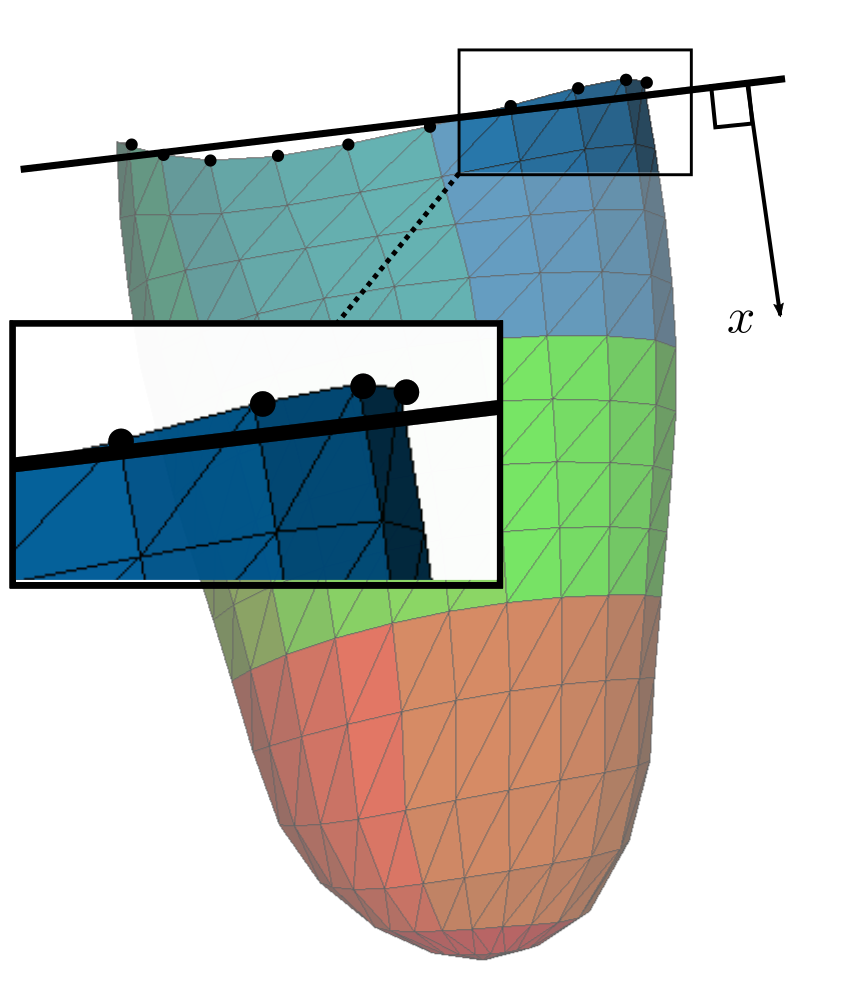
\includegraphics[width=\textwidth]{chapters/introduction/figures/geometry/strain_mesh_plane.pdf}
    \caption{\label{fig:strain_mesh_plane}}
  \end{subfigure}
  \begin{subfigure}[t]{0.45\textwidth}
    \includegraphics[width=\textwidth]{chapters/introduction/figures/geometry/cut.png}
    \caption{\label{fig:cut}}
  \end{subfigure}
\caption{}
\label{fig:echopac_output}
\end{figure}



The actualy mesh generation is performed using Gmsh
\cite{geuzaine2009gmsh}, which meshes the endocardial and epicardial
surface togther unsing frontal-Delaunay meshing algorithm. Gmsh also marks
the endocardal, the epicardial  and the basal facets, along with the
endocardial 

\begin{figure}[htbp]
  \centering
  \begin{subfigure}[t]{0.4\textwidth}
    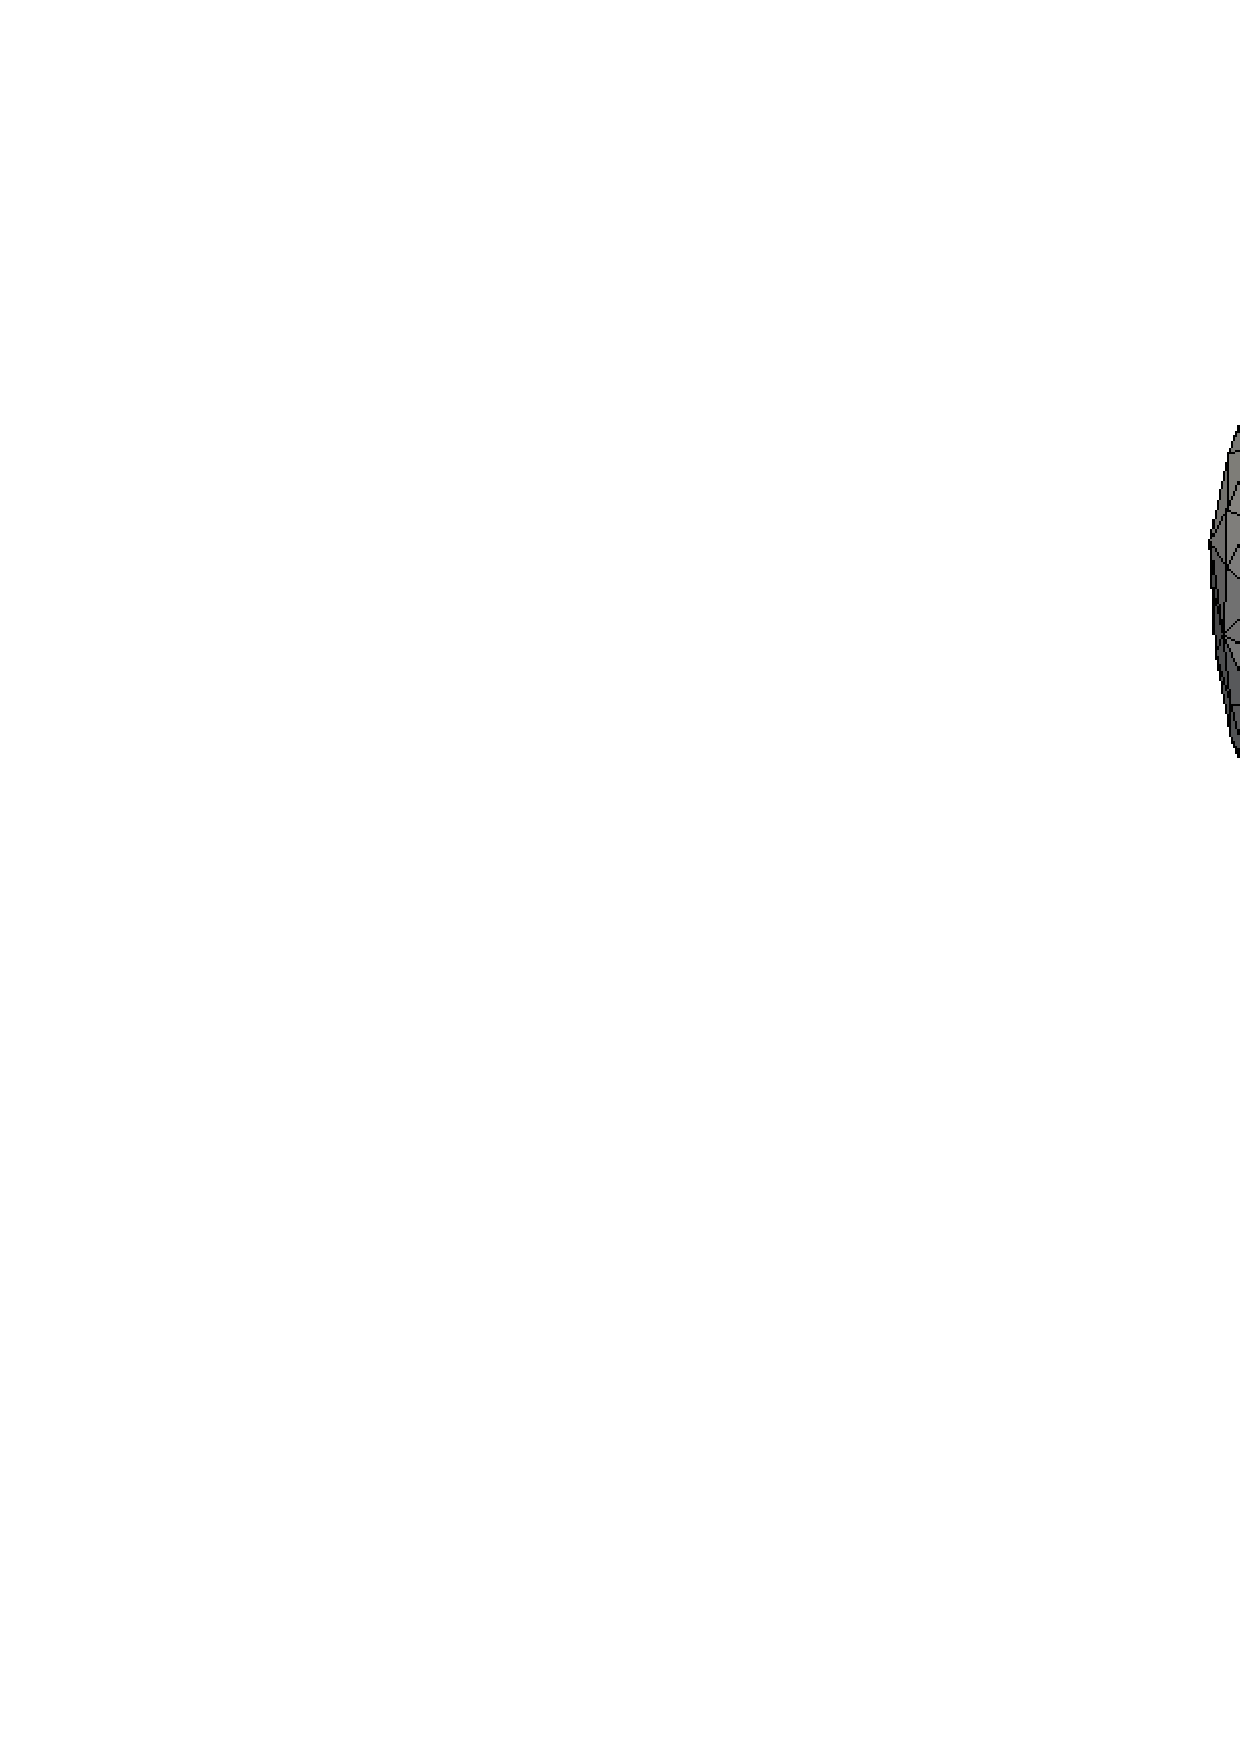
\includegraphics[width=\textwidth]{chapters/introduction/figures/geometry/mesh.png}
    \caption{\label{fig:mesh}}
  \end{subfigure}
  \begin{subfigure}[t]{0.45\textwidth}
    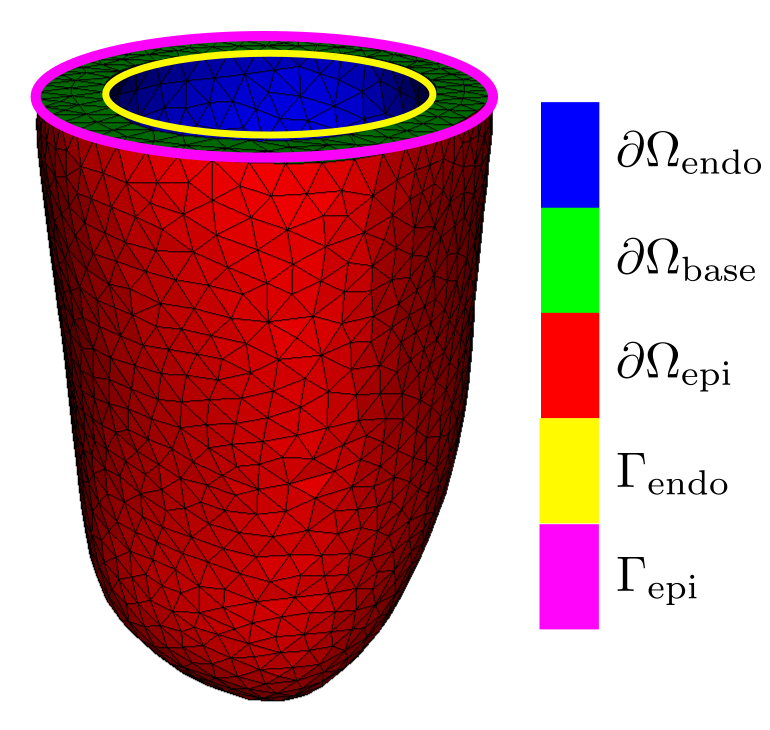
\includegraphics[width=\textwidth]{chapters/introduction/figures/geometry/markers_full.pdf}
    \caption{\label{fig:markers_full}}
  \end{subfigure}
\caption{}
\label{fig:echopac_output}
\end{figure}



\begin{remark}
  The cavity volume is computed by generating the whole mesh, and the
  compute the volume using Equation \eqref{eq:volume_operator}. The cut size is
  found by using a one dimensional optimization algorithm with
  the objective funcitonal representing the squared error between
  computed and measured volume.
\end{remark}




\subsubsection{Rule-based fibers}
\label{sec:rule_based_fiber}
Mention papers about fiber distribution, fiber dependence and
different rule-based fibers.

Describe the main steps in the Bayer algorithm. 


\subsubsection{The ventricular coordinate system}

When dealing with geometric shapes such as a left ventricle, finding a
coordinate system that is easy to work with is important. For
example, when studing spherical shapes, the spherical coordinate system is
usually easier to work with. Likewise, a coordinate system that is
easy to use when studying ellipsoidal shapes like the left ventricle is
the \emph{prolate spheroidal coordinate system} \cite{hunter1996kd}. 
The cartesian coordinates $(x,y,z)$ are related to the prolate
spheroidal coordinates by

\begin{align}
  \begin{split}
    x &= a \sinh \mu \sin \nu \cos \theta  \\
    y &= a \sinh \mu \sin \nu \sin \theta  \\
    z &= a \cosh \mu \cos \nu,
  \end{split}
\end{align}
where $a$ is the focal point, $\nu \in [0, \pi]$ is the longitudinal
coordinate, $\theta \in [0, 2\pi]$ is the azimuthal angle and $\mu$
is the radial coordinate. For an ellipse given by the equation
$\frac{x^2}{b^2} +\frac{y^2}{c^2}  = 1$ with $b$ being the semimajor
axis, and $c$ the semiminor axis, the focal point is given by
\begin{align}
  a =\sqrt{b^2 - c^2}.
  \label{eq:focal_point}
\end{align}
Assuming the ventricle is axisymetric around the
longitudinal axis, which is aligned with the $x$-axis it is possible
to estimate the focal point by taking $b$ in \eqref{eq:focal_point} to
be the maximum distance from the base to the apex, and $b$ the maximum
radius at the based. Using this estimate, the base is assumed to be
located approximately at the center of the ellipsoid, i.e $\nu = \pi /
2$. Compared to geometries used in benchmarking of cardiac mechanics
problems, this is not a totally wrong assumption
\cite{land2015verification}



\begin{figure}[htbp]
  \centering
  \begin{subfigure}[t]{0.4\textwidth}
    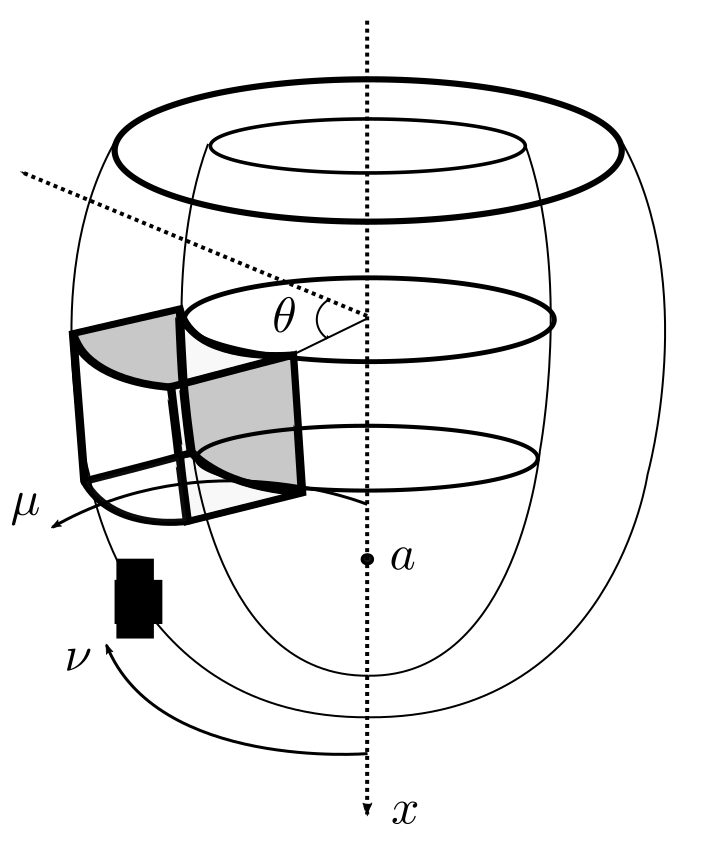
\includegraphics[width=\textwidth]{chapters/introduction/figures/geometry/prolate.png}
    \caption{\label{fig:prolate_coord}}
  \end{subfigure}
  \begin{subfigure}[t]{0.45\textwidth}
    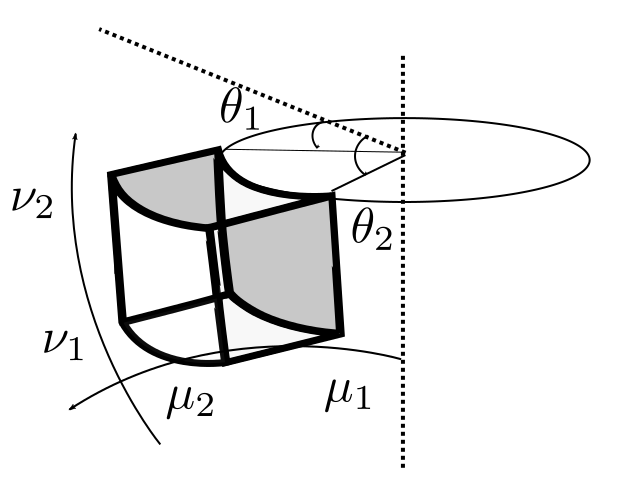
\includegraphics[width=\textwidth]{chapters/introduction/figures/geometry/prolate_cube.png}
    \caption{\label{fig:prolate_cube}}
  \end{subfigure}
\caption{}
\label{fig:prolate}
\end{figure}

\subsubsection{Marking the mesh according to the AHA-segments}



\begin{itemize}
  \item Segmentation and aquisition using echopach
  \item From closed endo- and epicardial surfaces to a mesh
    (smoothing, cutting, orienting).
  \item Marking of mesh accoring to AHA segments (16,17,18)
  \item Local basis
  \item Rule based fibers
  \item Referece to mesh{\_}generation and patient repositories
  \end{itemize}


\subsection{Data Assimilation}
The constitutive laws in cardiac mechanics comes from experiments
done on tissue slabs, and relates stresses in the material to strain.
If we had the same data available for a given patient we could easily
have performed a regression analysis in order to identify the
parameters in the contitutive model. However, this type of data
typically requires that tissue samples are taken from the myocardium,
which is not an option when dealing with living humans. In general,
when dealing with physical system such as the heart or weather
forecast it is not allways possible to design an experiment which
allows to determine all properties of a physical system
\cite{chapelle2013fundamental}. In such cases we have to take the
measurement that we have, and do our best to incorporate them into the
model. 

For example, the type of data that we usually have available, are data
that can be extracted using imaging techniques such as motion data,
volume traces, regional strain traces etc. One technique to estimate
model parameters based on such observations is called data assimilation.


The field of data assimilation has its roots in meteorology, where
a typical problem is to make predictions on the weather, based on
observations (of temperature, humidity etc.) at different locations. 


There are basically two main approaches to assimilate data;
\emph{sequential data assimilation} and \emph{variational data
  assimilation}. Sequential data assimilation, which is often
referred to as filtering, is based on a predictor-corector approach
where you start from your initial data and use a filter to predict the
next state. Once you have your measurement available you correct the
estimate based on the new observations. Some examples of sequential
procedures include Kalman filtering and Luenberger observers
\cite{chapelle2013fundamental}.

The other approach called variational data assimilation, which is the
one used in this thesis, is based on minimizing a cost functional that
represents the mismatch between observations and simulations, with
possibly additional regularization terms added to the objective
functional. 

% The general setup for a variational data assimilation problem is the
% following. 
We will now explain the general setup for variational data
assimilation. In order to keep consistent notation we will refer to
the \emph{state variable} as $\mathbf{w}$, which is our case
represents jointly the displacement and hydrostatic pressure
$\mathbf{w}=(\mathbf{u}, p)$.

The state varibles are described by some \emph{phyiscal
model} $\mathcal{L}$, which is our case is governed by the force balance
equations \eqref{eq:force_balance}, and can be written in the form
$\mathcal{L}\mathbf{w} = f$.

We are also given a set of measurements (or observations) that we want
to assimilate, and we denote this by the vector $\mathbf{y}$.
For example, $\mathbf{y}$ might be a set of volume measurements or a
combinations of volume and strain at given time points in the cardiac
cycle. The \emph{observation operator} $\mathcal{H}$, is approximation
of the observation and act as an operator from the state space to the
observation space. We therefore have the relation
\begin{align}
  \mathbf{y} = \mathcal{H}(\mathbf{w}) + \xi_o, 
\end{align}
where $\xi_o$ represents both the error in the measurements (e.g
noise in the data) and error in the representation of the observation
(that $\mathcal{H}$ do not represent the data good enough).


\paragraph{The volume observation operator
  $\mathcal{H}_{\mathrm{volume}}$}
In some cases, the ventricular cavity volume can easily be computed
analytically from the displacement field. Denote the inner cavity of
the left ventricle in the current configuration by
$\omega_{\mathrm{endo}}$. Further let $\mathrm{d} v$ and $\xvec$
denote an infinitesimal volume element and the coordinate in the
current configuration respectively. Then by the divergece theorem we have
\begin{align}
  \mathcal{H}_{\mathrm{volume}}(\uvec)= \int_{\omega_{\mathrm{endo}}} \mathrm{d} v =
  \frac{1}{3}\int_{\omega_{\mathrm{endo}}} \nabla \cdot \xvec \mathrm{d} v =
  \frac{1}{3}\int_{\partial \omega_{\mathrm{endo}}} \xvec \cdot \mathbf{n} \mathrm{d} s, 
\end{align}
where $\mathbf{n}$ and $\mathrm{d} s$ are the unit normal and a surface
element on the current configuration respectively.
Note that the boundary $\partial \omega_{\mathrm{endo}}$ includes the
endocardial basal boundary. However in the case when the base is flat
and fixed in longitudinal direction, the contribution from this
boundary integral will be zero. In this case the boundary integral
will be the same as the integral over the endocardial boundary
decribed in \ref{refer_to_section}, with the only change being the
change of sign on the normal vector. By Nansens formula we obtain
\begin{align}
  \mathcal{H}_{\mathrm{volume}}(\uvec)= -\frac{1}{3}\int_{\lvendo} \left( \Xvec + \uvec \right) J \F^{-T} \Nvec \mathrm{d}S,
  \label{eq:volume_operator}
\end{align}
where now $\lvendo$,  $\Xvec$, $\Nvec$ and $\mathrm{d}S$ are respectively the
endocardial surface, the referece coordinate, the unit normal and a
surface element in the reference configuration.


\paragraph{The strain observation operator
  $\mathcal{H}_{\mathrm{volume}}$}
Another observation that is encountered in this thesis is strain
measurements, of more precisely average regional strain in the
circumferential, radial or longitudinal direction. Let $\Omega_j$
denote the volume for which the strain should be averaged over, and
let $\mathbf{e}_k$ denote the unit vectorfield in the preferred strain
direction. Then for a given strain tensor $\mathbf{A}$ we define 
\begin{align}
  \mathcal{H}_{\mathrm{strain}}(\uvec) = \frac{1}{|\Omega_j|}\int_{\Omega_j} \mathbf{e}_k^T \mathbf{A}(\uvec) \mathbf{e}_k  \mathrm{d}V
\end{align}
The strain tensor $ \mathbf{A}$ is typically chosen to be the
Grenn-Lagrange strain tensor $\mathbf{E}$\eqref{eq:green_lagrange}, or
the material displacement gradient tensor $\F - \I$.

\begin{remark}
  Measured strains are computed relative to some reference
  geometry, which do not always coinside with the reference geometry
  chosen for your simulation. In these cases you have to either
  recompute the measured strain according to the chosen referece for
  the simulation, or recompute the simulated strains according to the
  correct referece geometry for your measuments. 
\end{remark}

% Within varitaional data assimilation it is common to separate between
% dynamic models and static models. These are conventionally reffered to as
% $4D-$Var and $3D-$Var methods respectively. In the work done this
% thesis we have used both of these methods. 


% For an introduction to data assimilation we refer to e.g \cite{lahoz2010data}.

Let us assume that 


\begin{itemize}
  \item Examples of data you want to constrain
  \item Forming of mismatch functional and problem formulation as
    PDE-constrained optimization.
  \item The adjoint approach. comparison with other methods.
  \item Control parameters
  \item OPtimization algorithm - stopping criteria
  \item Reference to pulse{\_}adjoint and pulse{\_}adjoint{\_}post
    repositories
  \item Variational versus sequnetial
  \item Question about uniquness
\end{itemize}


We will now explain what we mean by ``adjoint-based'', and why this
approach is a key ingredient. The main theory presented here is taken
from the dolfin-adjoint web page. A word about dolfin adjoint...\ref{}
  
\begin{equation}
  \begin{aligned}
    \label{eq:opt_matparam}
    & \underset{\mvec}{\text{minimize}}
    & &  \mathcal{J}(\state, \mvec) \\
    & \text{subject to}
    & & \delta \Pi(\state, \mvec) = 0, 
  \end{aligned}
\end{equation}

where $\mathcal{J}(\state, \mvec): \mathbb{W} \times \mathbb{Q} \mapsto
\mathbb{R}$ for some state space $\mathbb{W}$ and parameter space
$\mathbb{Q}$ and $\delta \Pi(\state, \mvec)) = 0$ is the force balance
equation given by \ref{}.
$\mvec = (m_1, \cdots m_P)$


Now suppose we have discretized the partial differental equation
$\delta \Pi(\state, \mvec) = 0$, which reduces to a system of the form
$\mathbf{A} \state = \mathbf{b}$, with possible all terms depending on
the parameters $\mvec$. The gradient of the cost functional with
respect to the parameter is given by
\begin{align}
  \frac{\mathrm{d} \mathcal{J}}{\mathrm{d} \mvec} = \frac{\partial \mathcal{J}}{\partial \mvec}
  + \frac{\partial \mathcal{J}}{\partial \state} \frac{\mathrm{d} \state}{\mathrm{d} \mvec}.
  \label{eq:grad_cost}
\end{align}
Here $\frac{\mathrm{d}}{\mathrm{d} \mvec}$ denotes the total
derivative, while $ \frac{\partial}{\partial \mvec}$ denotes the
partial derivative. Computing the partial derivatives in
\eqref{eq:grad_cost} are usually straight forward, while computing  $
\frac{\mathrm{d} \state}{\mathrm{d} \mvec}$ is hard. To see this, let
us differentiate the equation $\mathbf{A} \state = \mathbf{b}$ with
respect to $m_i$, and solve for the 


\begin{remark}
  In data assimilation we typically want to copmute the gradient of
  the cost function because we want to employ gradient-based
  optimization algorithms for finding the ``optimal'' parameter
  set. In other cases, the gradient might be important because it
  tells you something about the sensitivity of your function of
  interest with respect to the parameters. For example, if you have a
  model with many input parameters, you may want to identify what
  impact the different parameters has on the output. Perturbing each
  parameter and observing the chane in the objective function quickly
  becomes infeasible when the number of parameters becomes large, in
  which case the adjoint aproach offer a possible solution. 
\end{remark}



\subsubsection{Adjoint method}
In order to apply optimisation algorithm...
We reduce the objective functional to be a function of the control
parameters only, $\hat{I}(\mvec) := I(\state(\mvec), \mvec)$. Consider an
initial value of the parmameters $\mvec = \mvec^0$. If $\hat{I}(m)$ is defined
and differentible in a neighborhood of $\mvec^0$ then $\hat{I}$ (and
consequently $I$) decreases fastest in the direction of the gradient, 
\begin{align}
  \nabla_{\mvec} \hat{I}(\mvec^0) = \begin{bmatrix}
    \frac{\mathrm{d} \hat{I}(\mvec^0) }{\mathrm{d} m_1},
    \frac{\mathrm{d} \hat{I}(\mvec^0) }{\mathrm{d} m_2},
    \cdots
    \frac{\mathrm{d} \hat{I}(\mvec^0) }{\mathrm{d} m_N}
  \end{bmatrix}^T.
  \label{eq:functional_gradient}
\end{align}
Here $\frac{\mathrm{d} \hat{I} }{\mathrm{d} m_i}$ represents the
total derivative:
\begin{align}
  \frac{\mathrm{d} \hat{I} }{\mathrm{d} m_i} = \frac{\mathrm{d} I (\state(\mvec), \mvec))}{\mathrm{d} m_i} = \frac{\partial  I }{\partial \state} \frac{\mathrm{d} \state}{\mathrm{d} m_i} + \frac{\partial  I }{\partial m_i}.
  \label{eq:functional_derivative_component}
\end{align}
In other words, the sequence
\begin{align}
  \mvec^{k+1} = \mvec^{k} - \gamma_k \nabla_{\mvec} \hat{I}(\mvec^k), \gamma_n \in \mathbb{R}
\end{align}
satisfies $\hat{I}(\mvec^{k+1}) \leq \hat{I}(\mvec^k) \; \forall k \geq
0$, and converges towards a local minimum. If $\hat{I}$ is convex then
the minimum is also global.
Being able to compute the gradient of the objective functional wrt to
the control parameters allows us to employ gradient based optimization
methods which are in general superior to gradient free methods.
One way to compute the gradient is by means of the finite difference
approach: For a given parameter $\mvec = \mvec^*$ we have
\begin{align}
  \frac{\mathrm{d} \hat{I} }{\mathrm{d} m_i}( \mvec^*) =
  \lim_{h \mapsto 0} \frac{\hat{I}(\mvec^* + h\mathbf{e}_i) - \hat{I}(\mvec^*)}{h}, 
\end{align}
where $\mathbf{e}_i \in \mathbb{Q}$ is the $i$'th canonical basis
vector. If $\dim(\mathbb{Q}) = N$, this approach would require $N+1$
functional evaluations. Moreover, since the state-variables depends upon the
control variables, we would also need to solve the force balance
equation $N+1$ times, which is typically very copmutationally
expensive. Hence, this approach is typically infeasable when the
dimesion of your parameterspace is large. In this case the adjoint
approach is much better. If $A$ is an operator (e.g a matrix), then
the adjoint operator $B$ satisfies the relation $\langle Au, v \rangle
= \langle u, Bv \rangle$, and we write $ B = A^*$. Here $(\cdot)^*$
denotes the Hermitian transpose, which in the case where $A$ is a real
matrix is just the transpose of $A$, $A^T$.  


Note that the gradient in
\eqref{eq:functional_gradient} can be rewritten (using the chain rule)
as
\begin{align}
  \nabla_{\mvec} \hat{I} =  \frac{\partial  I }{\partial \state} \nabla_{\mvec} \state
  + \frac{\partial  I }{\partial \mvec},
  \label{eq:functional_gradient_chain}
\end{align}
in which the $\dim(\mathbb{V}) \times \dim(\mathbb{Q})$ matrix
$\nabla_{\mvec} \state$ is difficult to compute.
Differentiating the force-balance equation \ref{} with respect to the
control parameters yields
\begin{align}
  & \nabla_{\mvec} \delta \Pi(\state, \mvec) = 0 \\
  \implies & \frac{\partial  \Pi }{\partial \state} \nabla_{\mvec} \state
  + \frac{\partial  \Pi }{\partial \mvec} = 0 \\
  \implies & \nabla_{\mvec} \state =
             - \left( \frac{\partial  \Pi }{\partial \state} \right)^{-1} \frac{\partial  \Pi }{\partial \mvec}.
\end{align}
Inserting this expression for $\nabla_{\mvec} \state$ into
\eqref{eq:functional_gradient_chain}, gives
\begin{align}
  \nabla_{\mvec} \hat{I} =  - \frac{\partial  I }{\partial \state}
  \left( \frac{\partial  \Pi }{\partial \state} \right)^{-1} \frac{\partial  \Pi }{\partial \mvec}
  + \frac{\partial  I }{\partial \mvec}.
\end{align}


\subsubsection{Dolfin-Adjoint}

Dolfin-Adjoint is a software package that based on the FEniCS project
which aims to derrive the discrete adjoint equation and the tangent
linear models of finite element models implemented within the FEniCS
framework. While the tradional approach is to derrive the adjoint code
from the forward code using automatic differentiation tools,
Dolfin-Adjoint utilises the high level symbolic representation
\cite{UFL} in FEniCS to derrive the discrete adjoint equations from
the discrete forward eqations, and then the FEniCS system derrives the
adjoint code from the discrete adjoint equations. 

\subsubsection{Optimization methods}

Line search methods, interior point methods, gradient based methods,
genetic methods, trust region



\subsection{Identifiability of parameters}
% Try dividing heart mesh is different segment, discuss uniqueness of
% paraperers
% Discuss regularization technices
When dealing with parameter estimation, you should always consider
questions about identifiability and uniquness. This depends on the
model, the data and the objective functional
\cite{hadjicharalambous2015analysis}. A first test should be to
generate synthetic data with some prescribed parameters, feed this
error-free data to the data assimilation method, and ensure that you
are able to retrieve the parameters that generated that data. If you
end up with a different parameter set than the one generated the data,
your problem is not \emph{structuraly identifiable}
\cite{chabiniok2016multiphysics}. Your problem is said to be
\emph{practical identifiable} if the parameters can be determined
uniquely based on the data at hand. If the test passes you shold try
to add noise to the data, and see if your data assimilation is stable
with respect to noise in the measurement, and you should quantify the
model out error versus the model input error. Demonstrating identifiability is
often difficult, especially when your data is corrupted with noise,
and when the complexity of the model increases. Balancing the
complexity of model in terms of \emph{model fidelity}, i.e wheter your
model is rich enough to representing the data, and the identifiability
is often key in order to have robust model. A too simple model will
often fail to represent your data, while a too complex model, might
give completely differet answers with just a slight perturbation of
the data, i.e with noise added to the measurement. The same problem is
encountered in other scientific disiplines, for instance in
statistical learning theory, \emph{overfitting} is related to
overparameterization of the model, in which you can perfectly
represent your data, but a small perturbation will cause a significant
error. Another problem, which is also related to identifiability is
the question about uniquness of the soluton. A practical test is to
start the optimization algorithm from different intial points and see
if you end up at the same optimum. If this does not happen, it is
likely that the objective functional is not convex, which is a
requirement for uniquness. Unfortunately, this is the case for many
problems in PDE-constrained optimization. In these cases, the objective
functional might have several distinct local minima, in which case
different techniques for find the best local minima exists
\cite{farrell2015multiple}. 

\subsubsection{An example of a non-structuraly identifiable problem}
Split the ventricle in two, and use volume as the only input.
Show that differnt parameter sets (with $\gamma$) will generate the
same volume



\subsubsection{Material parameter estimation}

\paragraph{One volume measurement only}

\paragraph{Multiple volume measurements}

\paragraph{Volume and strain measurements}

\subsubsection{Coupled unloading and material parameter estimation}
In Section \ref{sef:reference_geometry} we described a method for
finding the uloaded configuration unsing the backward displacement
method. The problem of using this method when dealing with parameter
estimation is that the unloaded geometry depends on the material
properties, which in general is unknown. Hence we need a way of
estimating both the unloaded geometry and the material parameters at
the same time. One possibible algorithm is the following:



\begin{algorithm}
\caption{Coupled Unloading and material parameters estimation}\label{alg:unloaded_material}
\begin{algorithmic}[1]
  \State $i = 0$
  \State residual = $\infty$
  \State $\mvec_0 =  \mvec$ \Comment{Initial guess for material parameters}
  \While{i $<$ N and residual > tolerance }

  \State $\Omega_{\mathcal{U}}^i$ = Unload($\Omega_{\mathcal{I}}, \mvec_i$) \Comment{unload
    material}
  \State $\mvec_{i+1}$ = EstimateMaterial($\Omega_{\mathcal{U}}^i,
  \mvec_i$) \Comment{estimate material parameters}
  \State residual = ComputeResidual($\Omega_{\mathcal{U}}^i,
  \Omega_{\mathcal{U}}^{i-1}$)
  \State $i = i +1$
 
  \EndWhile
\end{algorithmic}
\end{algorithm}

\subsection{Activation parameter estimation}



\subsubsection{Multiobjetive optimization}
Paramaters in the model are estimated based on minimizing a cost
functional representing the mismatch between observations and simulaton.
Assume we are given $N$ different observations, then in priciple we
have $N$ different cost funcitonals to solve
\begin{equation}
  \begin{aligned}
    \label{eq:multiobjetive_opt}
    & \text{minimize}
    & &  \left\{ \mathcal{J}_1(\lambda), \mathcal{J}_2(\lambda), \cdots, \mathcal{J}_N(\lambda) \right\} \\
    & \text{subject to}
    & & \delta \Pi(\state(\lambda)) = 0, \lambda \in \mathcal{P},
  \end{aligned}
\end{equation}
whith 
\begin{align}
  \mathcal{J}_i(\lambda) = \left( \mathbf{y} - \mathcal{H}(\state(\lambda)) \right)^2, \; i = 1,\cdots, N
\end{align}
The above observations comes from the same soure, and hence it should
be intuitive that minimizing one of them, would also bring the other
closer to a minimum. However, with precense of noise in the data,
this might not always be the case, and hence we have a conflicting
objectives. Problem \eqref{eq:multiobjetive_opt} is called a
multiobjetive optimization problem \cite{deb2016multi}. Such problems
typically do not have a single optimal solution, but a family of
solutions called \emph{Pareto optmal solutions}. The basic methods for
solving such problems inclues \emph{the weighted method}, \emph{the
  $\varepsilon$-constraint method}, 




\subsection{Mehcanical biomarkers}
A word about what models can contribute with




%%% Local Variables:
%%% mode: latex
%%% TeX-master: "../../main"
%%% End:


\section{Summary of papers}
\label{sec:summary}
In this final introductory section we summarize the papers that make
up this thesis, and we also give some final concluding remarks
and future directions. 

\subsection{Paper 1: High-resolution data assimilation of cardiac mechanics
  applied to a dyssynchronous ventricle}



\begin{figure}[htbp]
  \centering
    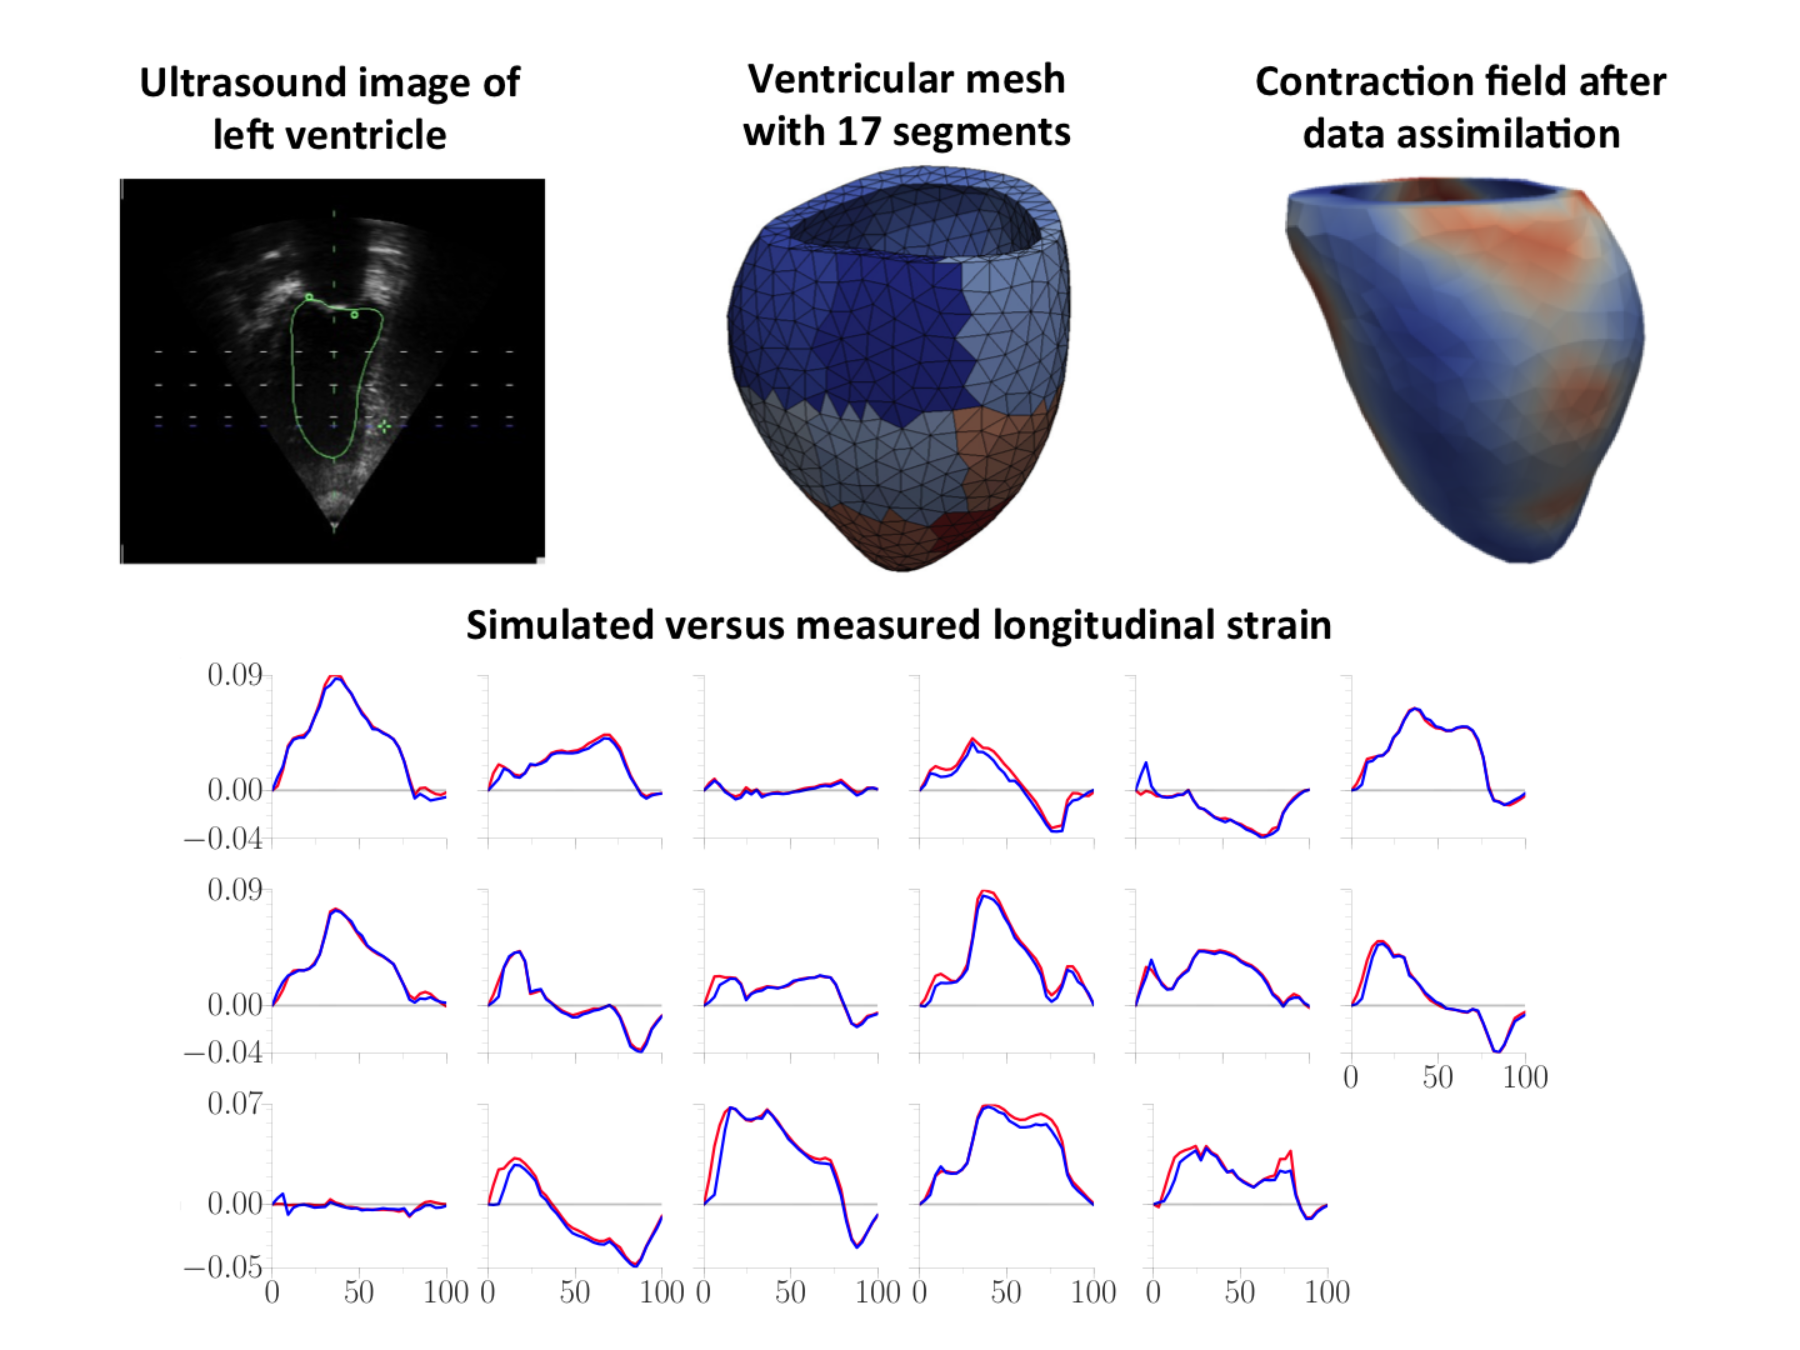
\includegraphics[width=0.8\textwidth]{chapters/introduction/figures/paper1}
\caption{Summary figure for paper 1}
\label{fig:paper1}
\end{figure}


In this paper we develop and test the pipeline for constructing a
patient specific mechanical simulation of a patient's heart, based on
clinical measurments and adjoint-based data assimilation
techniques.

As a model case we consider one patient, diagnosed with
left bundle branch block and selected for cardiac resynchronization
therapy (CRT). Prior to the CRT implantation the patient had 4D
echocardiography taken for which the LV geometry, LV volumes and LV
regional strains throughout the cardiac cycle are measured. During
implantation of the CRT device the LV pressure where also measured
invasively. The LV pressure measurements are used as boundary condition at the
endocardium, while the LV volume and LV regional strain is incorporated
into a cost functional that we want to minimize.


The pipeline is divided into two phases, a passive phase where we
estimate the linear isotropic parameters $a$ in
\eqref{eq:holzapel_trans} as a global material parameter using the
measurement points belonging atrial systole, and an active phase where we estimate the
a spatially varying contraction parameter ($\gamma$ in
\eqref{eq:intro_active_strain_Fa_gjerald}) at each measurement point
with active contraction. During the passive phase we only fit the
volumes, while during the active phase 51 strain measurements in the radial,
longitudinal and circumferential direction in each AHA segment (Figure
\ref{fig:echopac_output}) are used in the optimization. 

The results show an excellent fit with measured strain an volume, with
a average relative error in the volume and strain of less than 0.4 \% and 3 \%
respectively using a contraction parameter with one degree of freedom
for each vertex in the geometry (2661 parameters in total). Parameters
at lower spatial resolution are also tested to show the necessity of
high spatial resolution to fit the measured strain data.
A synthetic test is also performed in order to show that that method
is able to recapitulate the generated data, also with noise added to
the data. Moreover, a sensitivity analysis to different parameters are
presented in the appendix.


\subsection{Paper 2: Estimating cardiac contraction through high resolution
  data assimilation of a personalized mechanical model}


\begin{figure}[htbp]
  \centering
    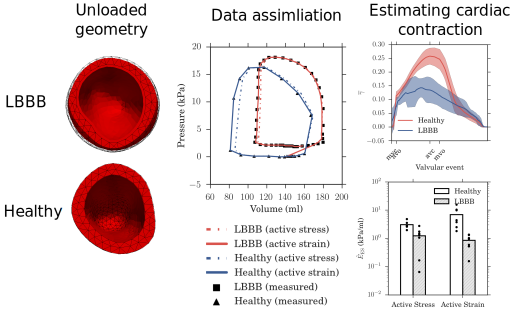
\includegraphics[width=0.8\textwidth]{chapters/introduction/figures/paper2}
\caption{Summary figure for paper 2}
\label{fig:paper2}
\end{figure}

In this paper we apply the method developed in the previous paper to a
cohort of patients and estimate indices of cardiac contractility. More
specifically, a group of seven patients diagnosed with left bundle branch block and
selected for cardiac resynchronization therapy (CRT) and a group of
seven healthy control subjects where included in the study.

The pipeline is similar to the one outlined in paper 1, with the
exception that we also estimate the unloaded, stress-free
configuration using the method outlined in Section
\ref{sec:intro_coupled_material}. 

The optimized active strain parameter in
\eqref{eq:intro_active_strain_Fa_gjerald} as well as the optimized
active stress parameter in \eqref{eq:intro_active_stress} are averaged
over the ventricle and compared between the two groups. The healthy
group showed a significant increase in both of these
parameters. Furthermore, estimation of end-systolic elastance by
perturbation of the pressure at the end-systolic state while fixing
the remaining quantities were made. This estimate of end-systolic
elastance where also significantly higher in the healthy control
group. 


\subsection{Paper 3: Personalized bi-ventricular mechanical analysis
  using gradient-based optimization..}

\begin{figure}[htbp]
  \centering
    \includegraphics[width=0.8\textwidth]{chapters/introduction/figures/paper3}
\caption{Summary figure for paper 3}
\label{fig:paper3}
\end{figure}

In this paper we extend the work in the two previous paper to
bi-ventricular geomtries, and use it to estimate patient-specific
myofiber stress and indices of contractility. Furthermore, we investigate
the senstivtiy of these computed features the helical fiber angle and
the choice of active modeling framework.

In this work we estimate the linear isotopic material parameter in
\eqref{eq:holzapel_trans}, spatially resolved on the LV and RV, by
minimizing the error in end-diastolic LV and RV cavity volumes. We also
apply a simplified algorithm for estimating in unloaded geometry, in
order to overcome issues related to estimating an unloaded
BiV-geometry, which is not well-posed. The amount of active
contraction is estimated during the active phase, by minimizing
simulated and meausured volumes and circumferential strain. The active
control parameter, which are $\gamma$ in
\eqref{eq:intro_active_strain_Fa_gjerald}  and $T_a$ in
\eqref{eq:intro_active_stress} for the active strain and active stress
formulation respectively, are spatially resolved on the
LV free wall (LVFW), the RV free wall (RVFW) and the septum. With so
few control parameters, issues related to conflicting objectives, i.e
that is is not possible to minimize both the strain and volume, is
evident. However, with a low dimensional parameter space, questions
regarding identifiability and uniqueness of the estimated parameters
are easier to answer. In this study we also perform a validation of
the model, by comparing simulated and measured longitudinal strain
which is not used in the optimization. 

The results show low variability with respect to choice of fiber angle
and active modeling framework. Also, the fit of data depends upon the
choice of fiber angle, and a steeper fiber angle than previously
suggested, provides the best fit. The work here could potentially be
used to extract patient-specific maps of ventricular fiber stress and
contractility which could be useful in diagnostic of several heart
diseases related to heart failure. 




\subsection{Paper 4: Assesment region regional myocardial work using
  adjoint-based data assimilation}

\newpage
\section{Other contributions}
Along with the research articles presented in this thesis, other
types of contributions in terms of talks, posters and software has
been made during the writing of this thesis. These contributions are
listed below.

\subsection{Talks}
\begin{itemize}
  \item Henrik Finsberg, Gabriel Balaban, Joakim Sundnes, Hans
    Henrik Odland, Marie Rognes, and Samuel T. Wall. ``Patient
    Constrained Ventricular Stress Mapping'',
    Conference Presentation at MALT 2015,  Lugano, Switzerland (2015).
  \item Henrik Finsberg, Gabriel Balaban, Joakim Sundnes, Marie
    Rognes, and Samuel T. Wall. ``Personalization of a Cardiac
    Compuational Model using Clinical Measurements'', Conference
    Presentation at 28th Nordic Seminar on Computational
    Mechanics. Vol. 28. Tallin, Estonia, (2015).
  \item Henrik Finsberg, Gabriel Balaban, Joakim Sundnes, Marie
    Rognes, and Samuel T. Wall. ``Optimization of a Spatially Varying
    Cardiac Contraction parameter using the Adjoint Method'',
    Conference Presentation at FEniCS 16, Oslo, Norway,(2016).
  \item Finsberg, Henrik N., Gabriel Balaban, Joakim Sundnes, Hans
    Henrik Odland, Marie Rognes, and Samuel T. Wall. ``Personalized
    Cardiac Mechanical Model using a High Resolution Contraction Field
    '',  Conference Presentation at VPH16 Translating VPH to the
    Clinic,  Amsterdam, Netherlands (2016).
\end{itemize}


\subsection{Posters}
\begin{itemize}
  \item Henrik Finsberg, Gabriel Balaban, Joakim Sundnes, Marie
    Rognes, and Samuel T. Wall. ``Patient Specific Modeling of Cardiac
    Mechanics using the Active Strain Formulation '',
    Geilo Winter School, Geilo, Norway, (2016).
  \item Henrik Finsberg, Ce Xi, J. Tan, L. Zhong, LC Lee, Joakim
    Sundnes, and Samuel T. Wall. ``Mechanical Analysis of Pulmonary
    Hypertension via Adjoint based Data Assimilation of a Finite
    Element Model '', Summer Biomechanics, Bioengineering, and
    Biotransport Conference, Tucson, AZ, (2017). 
  \end{itemize}


\subsection{Software}
\begin{itemize}
  \item Pulse-Adjoint, FEniCS-based cardiac mechanics solver and data
    assimilator, source: \url{https://bitbucket.org/finsberg/pulse_adjoint}
  \item Mesh-Toolbox, Toolbox for generating FEniCS meshes from 4D
    Echo,  source: \url{https://bitbucket.org/finsberg/mesh_generation}
\end{itemize}


\newpage
\section{Closing remarks and future directions}

Although we have shown in this thesis that
adjoint-based data assimilation is a powerful technique that opens new
possibilities in terms of patient specific mechanical simulations, many questions
still has to be answered before we can fully embrace the output of
such simulations.

First of all, is should be clear that \emph{the
  quality of biomarkers you can extract from a data-driven
  model cannot be any better than the data used as input to the
  model}. A typical saying is that garbage in $=$ garbage out,
meaning that if the data you use to constrain the model is noisy, then
you will also fit this noise if you allow for enough degree of
freedom. Regularization techniques (Section
\ref{sec:intro_regularization}) provides a way to attack this problem,
but it is not clear what is the best approach. If the noise in the
data is normally distributed with zero expected value, then adding
more data to the cost functional will also have a regularizing effect.
Hence, as the data assimilation techniques developed in this thesis
can take into account large amount of data, as much data as possible
should be provided to the assimilator.

A rule of thump is that \emph{the spatial resolution of the parameters should be
  reflected in the spatial resolution of the observations}. This means
that if one is trying to fit data that are spatially resolved at some level,
then choosing parameters that are resolved at a finer level should be
done with caution. Regarding both paper 1, 2 and 4 we see that the
spatial resolution chosen was at a much finer level than the input
data. In this case, regularization techniques was used to restrict the
parameter space. 



Regarding the mechanical modeling of the heart, 
\emph{choosing appropriate boundary conditions} that reflect the reality has
been an issue during the work of this thesis, and several different
choices has been made. Moreover, \emph{accounting for the orthotropic as
well as the visco-elastic behavior of the myocardium} is something that should
be investigated in future studies. Accounting for an orthotropic
behavior would acquire more parameters to be estimated, which would
thus require more input data.

In this thesis we have also not fully
explored the \emph{spatial resolution of the material parameters}, and it
should be investigated whether it is possible to relate locally estimated
tissue stiffness to e.g myocardial infarction.

% The choice of active model for the myocardium is another topic that
% should be addressed in more detail in future studies. In the author's
% opinion, the output of the two fundamentally different approaches may
% vary a lot. In particular, it is evident that the active strain
% formulation do a better job in fitting strain data. One
% hypothesis is that the amount of transverse active stresses should be
% adjusted to each individual. These transverse active stresses are
% naturally embedded in the active strain approach via a volume
% preserving active deformation.


Finally, when estimating high dimensional parameters, a natural question
concerning uniqueness of these estimates arises. It is obvious that if one allows for
enough degree of freedom in the parameter space, then it is possible
to fit almost any type of data. Therefore \emph{more work on ensuring
identifiability} of these estimates (Section
\ref{sec:intro_identifiability}) should be done. If the output of such
model should have any clinical utility, then uniqueness of the
estimated parameters is absolutely pivotal. Moreover, \emph{validation} of
these model is what matter most in terms of translating such computational
models into the clinic.
% Here we start by listing a couple of statements
% which should be taken into considerations. 


% \begin{itemize}
% \item \emph{The quality of features/biomarkers you can extract from a data-driven
% model cannot be any better than the data used as input to the
% model}. Most of the results presented in this thesis are based on data
% obtained from clinical measurements of real patients.
% \item \emph{The spatial resolution of the parameters should be
%     reflected in the spatial resolution of the observations.} When
%   trying to fit data that are spatially resolved at some level,
%   choosing parameters that are resolved at a finer level should be
%   done with caution. The continuity in the underlying physics as well
%   as regularization techniques could be used to ...

% \end{itemize}

% During the work of this thesis, several questions still remains open
% and would require

% \begin{itemize}
% \item The active model for the myocardium is has .. Degree of
%   tranverse activation. Matching of strain data..
% \item Identifiability of parameters... Uniqueness of
%   solutions.. Amount of regularization.. Convexity of the mismatch functional
% \item Appropriate boundary conditions.. In paper three we saw big
%   differences in the choice of boundary conditions. Especially, the
%   magnitude of the stress seems to 
% \item Coupling of electrophysiologigy and mechanics in an
%   ajoint-based. data assimilation framework. 
% \end{itemize}

%%% Local Variables:
%%% mode: latex
%%% TeX-master: "../../main"
%%% End:



\pagebreak


\bibliographystyle{plain}
\bibliography{chapters/introduction/bibliography}


%%% Local Variables:
%%% mode: latex
%%% TeX-master: "../main"
%%% End:
